\chapter{A brief introduction to electric charges, currents, fields and potentials}
\label{chap:Basics}
%%% fref fixed
\ghnote{Teksten er ganske ferdig naa. De stoerste inngrepene er (1) Torbjorns to Jumping up in spatial scale-kapitler er nye. Jeg likte dem, men har endret en del paa dem. (2) Slik Jumping-kapitlene sto, var det ene en egen "section", mens det andre var en "subsection", og det mislikte jeg. Jeg har derfor endret litt paa rekkefoelgen av delkapitler, for aa faa dem paa samme nivaa. (3) Laget en ny versjon av Torbjorns "interpreting the extracellular potential-kapittel". Trenger en gjennomgang. (4) Har endret her og der, og markert de mest banebrytende endringene med farget tekst. (5) Har gaatt over til $V$ for potensial, og foreslaar at $\phi$ er ut. (6) Figurene maa revideres, konvertere fra $\phi$ til $V$ og eventuelt annet. (7) Vi hadde brukt current continuity og current conservation om hverandre i samme mening. Jeg byttet alt til conservation. (8) Se paa kommentarer.}

Neural activity is generated by electric currents that go through neural membranes. These transmembrane currents give rise to electric potentials in the extracellular space of the brain. The main goal of this book is to explore the relationship between the extracellular potential and the underlying neural signaling. 

Before addressing the brain specifically, we will here give a general introduction to electromagnetic theory, focusing mostly on the electric part of it, and less on the magnetic. The aim of this rather incomplete introduction is to establish an elementary understanding of the main concepts that we will use in the remainder of this book.

Electromagnetic theory is summarized by Maxwell's equations, and we might have kick-started this chapter by listing up those. However, since Maxwell's equations may appear a bit challenging for "the untrained eye", we will be taking a "softer" path, which we deem sufficient for establishing the main concepts that we will be working with. For good taste and later reference, we nevertheless go through Maxwell's equations in the final part of the chapter (Section \ref{sec:Basics:Maxwell}). Towards the end of the chapter we will also go through some of the most important assumptions that we use when applying the electromagnetic theory to predict electric potentials in a complex medium like brain tissue.

Readers without prior schooling in physics might not be able to follow all parts of this introduction, but it will hopefully still give them a basic understanding of the concepts of \textit{electric charge}, \textit{electric currents}, \textit{electric fields}, and \textit{electric potentials}, and some insight into how they are related to one another. Readers that do have a physics background might see the first part of this introduction as a useful repetition, and may appreciate the later parts, which deal with less trivial issues regarding the use of electromagnetic theory in a complex medium such as brain tissue.



\section{\blue{Electric charge}}
\label{sec:Basics:Charge} \index{Charge}
Let us begin with the fundamental quantity for electricity, the electric charge. Nature's fundamental charges are those carried by the protons and electrons that build up the atoms that build up the material world. The proton carries the charge $e$, while the electron carries the charge $-e$, where $e = 1.602\times10^{-19}$ coulomb (\si{\coulomb}) is called the \textit{unit charge}\index{Unit charge}. A fundamental law of nature is {\it charge conservation}\index{charge conservation}, meaning that it seems fundamentally impossible to create or destroy a net amount of positive or negative charge. The universe as we know it is exactly electrically neutral, and atoms in their neutral state contain an equal number of electrons and protons.

Although most matter is electrically neutral, some mediums are nevertheless \textit{conductive}, which means that they contain so-called "free charge carriers" that may move through the medium. In an electric copper wire, such as that carrying current to a normal desktop lamp, the free charge carriers are electrons that are not bound to specific locations (i.e., to specific copper atoms), but can move freely through the copper material. In an electrolyte solution, for example salt water (saline), the free charge carriers are instead ions, i.e., atoms or molecules that have gained or donated one or several electrons, and therefore have become electrically charged. The saline solutions that fill the intracellular and extracellular space of the brain are such electrolytic solutions. Important charge carriers in the brain are sodium and potassium ions (Na$^+$ and K$^+$ with charge $1e$), chloride ions (Cl$^-$ with charge $-1e$), and calcium ions (Ca$^{2+}$ with charge $2e$).

At a fundamental level, electricity is due to the movement of single charges. Such movement can be caused both by electric and magnetic forces, \tvntxt{\sout{as well as diffusion}}\ghnote{Paa det fundamentale planet jeg tenkte meg her diffusjon et uttrykk for elektriske vekslvirkninger}. We start with the electric force, which is the most important for the phenomena that we will study in this book. According to Colulomb's law, a pair of charges, $q_1$ and $q_2$, will act on each other with a force $F$ (with units newton (\si{\newton})) given by:
\begin{equation}
F = \frac{q_1q_2}{4\pi \epsilon_0} \frac{1}{r^2},
\label{eq:Basics:CoulombF}
\end{equation}
where the constant $\epsilon_0$ is the permittivity of free space, and $r$ is the distance between the two charges. The direction of the Coulomb force is along the line between the two charges, and the force is inversely proportional to the square of the distance between them. The force will be repelling if the charges have the same sign and attractive if they have the opposite sign. 

We can express the direction of the force mathematically by use of a vector notation. Letting a boldface notation indicate that an entity is a vector, we denote the positions of the charges $q_1$ and $q_2$ by ${\bf r}_1$ and ${\bf r}_2$, respectively. The position vector ${\bf r}_1$ can be visualized as an arrow from some reference point ${\bf r} =0$ to the position of the charge $q_1$. Likewise, the vector ${\bf r}_1-{\bf r}_2$ can be visualized as an arrow from the position of $q_2$ to the position of $q_1$, defining both the distance and direction of the (imagined) line connecting them. In vector notation, the force acting on the charge ($q_1$) by the charge ($q_2$) can be written:
\begin{equation}
{\bf F}_{1} = \frac{q_1q_2}{4\pi \epsilon_0 |{\bf r}_1-{\bf r}_2|^2} {{\bf e}}_{2,1}.
\label{eq:Basics:CoulombFvec}
\end{equation}
We have here introduced the \textit{unit vector},
\begin{equation}
{{\bf e}}_{2,1} = \frac{{\bf r}_1 - {\bf r}_2}{|{\bf r}_1-{\bf r}_2|},
\label{eq:Basics:UnitVector}
\end{equation}
defined as vector ${\bf r}_1-{\bf r}_2$ divided by its own length $|{\bf r}_1-{\bf r}_2|$, so that its length is one (unity). We chose this notation because the unit vector then defines the direction of the force in \fref{eq:Basics:CoulombFvec}, but says nothing about its magnitude, while the fraction in front of it is a scalar (a number with no direction) that defines the magnitude of the force, but  says nothing about its direction. It is then easy to verify that the magnitude is the same as in \fref{eq:Basics:CoulombF}.

If there are several ($N$) point charges present, the contribution from each of them to the total force sum up linearly. If we have a charge $q_1$ in a position ${\bf r}_1$, the force acting on it by the $N-1$ other charges $q_2, q_3, q_4 ... q_{N}$ in positions ${\bf r}_2, {\bf r}_3, {\bf r}_4 ... {\bf r}_{N}$ will be:
\begin{equation}
{\bf F}_1 = \sum_{n=2}^{N} \frac{q_1 q_n}{4\pi \epsilon_0} \frac{{{\bf e}}_{n,1}}{|{\bf r}_1-{\bf r}_n|^2}.
\label{eq:Basics:CoulombFN}
\end{equation}
Whereas a pairwise particle interaction was well described by the scalar expression in \fref{eq:Basics:CoulombF}, the summation of several force contributions acting in different directions could not be done without using a vector notation, as in \fref{eq:Basics:CoulombFN}.
\ghnote{Gaute spotta fortegnskluss her. Burde vaere i orden naa. Konvensjon paa hva ${\bf e}_{1,2}$ betyr - fra 1 til 2 eller motsatt, ser ut til aa variere. Hos oss betyr det naa FRA 1 TIL 2, og det samme er brukt for stroemmer i utledning av kavellingning i NEURON-kapittelet.}

If our system of study consisted of a small number $N$ of charges, we could use $N$ instances of \fref{eq:Basics:CoulombFN} to compute the force acting on all the $N$ individual charges. Together with Newton's law ${\bf F} = m {\bf a}$, which tells us how the charges will be accelerated in the force direction, \fref{eq:Basics:CoulombFN} would then allow us to compute the movements of all our charges over time. \ghtxt{For a macroscopic system, the number of charges involved is anything but small, and it not practically attainable to keep track of individual charges. As we will see later, the electrodynamics of macroscopic systems are instead studied using equations valid at a larger spatial scale. }

%However, the systems that we will be concerned with in this book consist of a very, very large number of charges, and keeping track of them individually by is not practically attainable. 


%Although \fref{eq:Basics:CoulombFN} establishes the fundamental origin for electric interactions, there is a fairly long way to go from this equation to the understanding of electric phenomena in a macroscopic system such as for example the brain. When describing a macroscopic system, we are usually not interested in the microscopic interactions between a small number of charges, but rather the joint interactions of a very, very large number of charges. It is then not feasible to keep record of the position of each individual charge, but rather to work with continuous variables defined on a larger spatial scale, such as charge densities, $\rho$ (with units \si{\coulomb\per\cubic\metre}), or ion concentrations, $c_k$ (with units millimolar ($1\, \si{\milli\molar} = 1 \,\si{\mole\per\cubic\metre} = 6.02\times10^{23}$ particles per \si{\cubic\metre})). The movement of particles of a given species $k$ is then quantified in terms of a particle flux, $J_k$, with units \si{\mole\per\second}, and the movement of charge is quantified in terms of an electric current, $I$, with units ampere (\si{\ampere} = \si{\coulomb\per\second}).
%\tvnnote{Kanskje ryddigere aa flytte dette avsnittet til litt senere, naar vi gaar over til stroemmer? Foelses litt uryddig aa saavidt nevne det her, men saa fortsette med enkelt-ladninger. Kan eventuelt begynne kapittelet med aa fortelle at vi skal til stroemmer og potensialer, men beggynner paa bunn og jobber oss oppover i skala}
%\gen{I tillegg kan det jo ogsaa vaere magnetiske krefter paa ladninger, kanskje bare nevne det for "completeness"?}
%\ghnote{La til kort kommentar i begynnelsen.}


\section{\blue{Electric fields and potentials}}
\label{sec:Basics:Fields} \index{Electric field}
The electric field at a given location (with units volts per metre (\si{\volt\per\metre})) can be defined as the electric force that \textit{would} act on a reference charge $q$ if it were present there, i.e.,
\begin{equation}
{\bf E}({\bf r}) = {\bf F}({\bf r})/q.
\label{eq:Basics:E}
\end{equation}
Since the electric force is due to the Coulomb force, the electric field generated by $N$ charges can be obtained by inserting \fref{eq:Basics:CoulombFN} into \fref{eq:Basics:E}:
\begin{equation}
{\bf E}({\bf r}) = \sum_{n=1}^{N}  \frac{q_n}{4\pi \epsilon_0} \frac{{{\bf e}}_{1,n}}{|{\bf r}-{\bf r}_n|^2}.
\label{eq:Basics:CoulombEN}
\end{equation}

Tightly related to the electric field ${\bf E}$ is the electric potential $V$ (with units volts (\si{\volt})), which is what we normally measure experimentally with electrodes.\index{Electric potential} Unlike ${\bf E}$, which is a vector field, $V$ is a scalar field, and as such, tends to be easier to deal with because measuring the value of a vector field requires measurement in all three spatial dimensions. The electric field is said to be conservative if it can be written as the gradient, or spatial derivative, of the potential:
\begin{equation}
{\bf E}(x,y,z) = - {\bf \nabla} V(x,y,z) = - \left(\frac{dV}{dx} {\bf e}_x  + \frac{dV}{dy} {\bf e}_y + \frac{dV}{dz} {\bf e}_z \right).
\label{eq:Basics:EV}
\end{equation}
The operator ${\bf \nabla}$ computes scalar field's spatial rate of change in the various spatial directions, and ${\bf e}_x$, ${\bf e}_y$ and  ${\bf e}_z$ are the unit vectors in the three spatial directions $x$, $y$ and $z$, respectively. We note that \fref{eq:Basics:EV} only holds when magnetic field variations are assumed to have negligible impacts on ${\bf E}$. As we shall see, this is an excellent approximation for the processes that we will study in brain tissue (see 
\fref{sec:Basics:Maxwell}).

For a spherically symmetric potential,
\begin{equation}
{\bf \nabla} V(r) = \frac{dV(r)}{dr} {\bf {e}}_r, 
\label{eq:Basics:SphericalNablaPhi}
\end{equation}
where ${\bf {e}}_r$ is the unit vector in the radial direction. Since the field contribution from each point charge is spherically symmetric around its position (${\bf r}_n$), the field in \fref{eq:Basics:CoulombEN} can be written as the gradient of the potential:
\begin{equation}
{V}({\bf r}) = \sum_{n=1}^{N}  \frac{q_n}{4\pi \epsilon_0} \frac{{{\bf e}}_{1,n}}{|{\bf r}-{\bf r}_n|}.
\label{eq:Basics:CoulombPhiN}
\end{equation}
In practical physics problems one rarely knows the positions of all present charges $q_n$, and the computation of the electric field from \fref{eq:Basics:CoulombEN} or the potential from \fref{eq:Basics:CoulombPhiN} can therefore only be done in idealized physics examples. Fields and potentials are nevertheless useful quantities at a systems level. They can be measured experimentally, and as we will come back to later, they can be computed from other physical principles than
interactions between individual charges.


\subsection{\blue{Reference point for potentials}}
\label{sec:Basics:Ground}
To get an intuitive understanding of the relationship between ${\bf E}$ and $V$, it helps to consider an idealized one-dimensional (1D) scenario with a constant field in the $x$-direction. Then, \fref{eq:Basics:EV} simplifies to,
\begin{equation}
E = -\frac{dV(x)}{dx} = -\frac{\Delta V}{\Delta x} = -\frac{V(x_b)-V(x_a)}{x_b-x_a},
\label{eq:Basics:EV1D}
\end{equation}
where the first equality follows from the 1D assumption, the second from the assumption that $E$ is constant, and the third is simply a definition of the second, where $x_b$ and $x_a$ may represent any two arbitrary points in space. For example, if $E = 1$~\si{\volt\per\metre}, and the distance between our points $x_b-x_a$ is 1~\si{\metre}, \fref{eq:Basics:EV1D} tells us that $V$ will be 1~\si{\volt} lower in $x_b$ compared to $x_a$ (\fref{fig:Basics:Ground}).

\begin{figure}[!ht]
\begin{center}
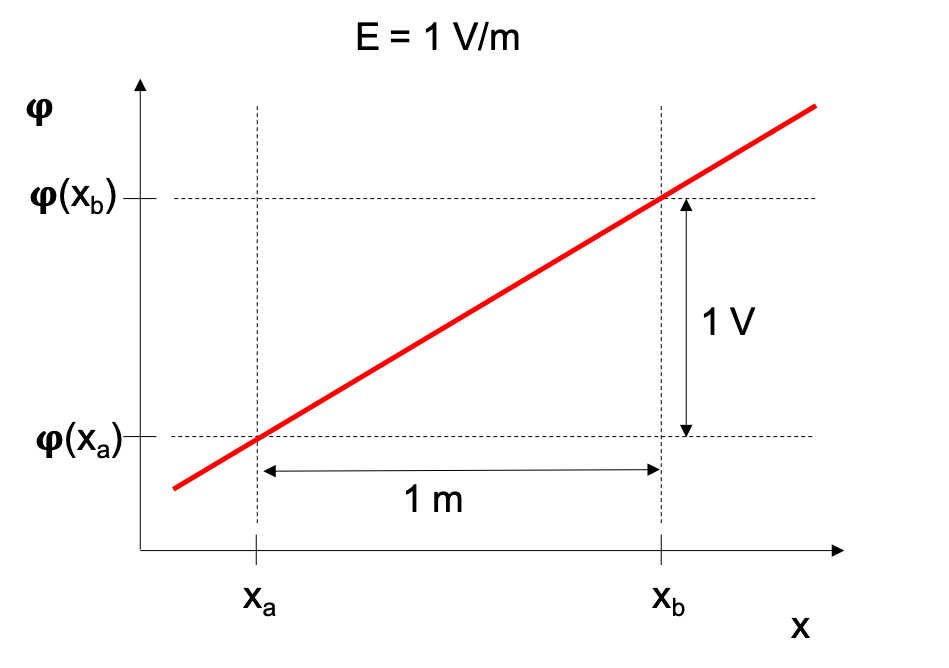
\includegraphics[width=0.8\textwidth]{Figures/Basics/Ground.png}
\end{center}
\caption{\textbf{Relationship between the electric field and electric potential.} With a constant electric field $E = 1\,\si{\volt\per\metre}$, the electric potential $V$ increases linearly with distance $x$. With two locations $x_a$ and $x_b$ 1~\si{\metre} apart, we know that $V(x_b) = V(x_a) + 1\,\si{\volt}$. We are free to define an arbitrary reference point (ground) for the $V$, and if we take $V(x_a) = 0$, it follows that $V(x) = (x-x_a)E$. In $x_b$, we then get $V(x_b)=(1\,\si{\metre})\times(1\, \si{\volt\per\metre}) =1\,\si{\volt}$. Equivalently, we might define $x_b$ as our reference point, which would mean that $V(x_b) = 0$ and $V(x_a) = -1\,\si{\volt}$. Regardless of where we place our reference point, the physics (i.e., the field, $E$) would be the same.
}
\label{fig:Basics:Ground}
\end{figure}

In the example, the field $E = 1\,\si{\volt\per\metre}$ would be consistent with any pair of potentials $V_a$ and $V_b$ as long as $V_b - V_a =  1 \,\si{\volt}$. Hence, the field ${\bf E}$ generally determines the potential only up to a constant. We can therefore not speak of the potential in a certain point as an absolute entity, but only the potential \textit{difference} between two points. When we measure the potential in a given location, it is always measured relative to some reference electrode that is placed in another location (\fref{fig:Basics:elec_circuit}), where we define $V = 0$ (cf. example in \Fref{fig:Basics:Ground}). 
When we record extracellular potentials in the brain, the optimal positioning of the reference electrode can be either close or far away from the recording electrode, depending on the kind of signal one wishes to measure \cite**{Sharott2015}.

\ghnote{Eventuell videre diskusjon om elektrodeplasseringer tas i VC-kapittelet, modeling the electrode.}


\subsection{\blue{Physical interpretation of the potential}}
\label{sec:Basics:interp_pot_charge}
By definition, the electric potential is the energy needed to move a unit of electric charge $q$ from the reference point (ground) to a specific location in the electric field (see \fref{sec:Basics:interp_pot_brain} for a illustrative example). The unit (\si{\volt}) of the electric potential is equivalent to energy per charge, or joule per coulomb (1 \si{\volt} = 1 \si{\joule\per\coulomb}). As such, the concept of an electric potential is closely related to the concept of a potential energy. The potential energy ($U_\text{E}$) of a charge $q$ in an electric field is:
\begin{equation}
U_\text{E} = qV.
\label{eq:Basics:UE}
\end{equation}


\subsection{\blue{Electroneutrality and Debye shielding}}
\label{sec:Basics:Debye}
Above, we saw that the electric potential resulting from a certain known arrangement of charges is given by \fref{eq:Basics:CoulombPhiN}. This formula works very well for textbook physics examples considering a few bound charges in a non-conducting material or in vacuum, but it is not very useful for studying processes taking place on a larger spatial scale in a conducting material, such as brain tissue. The reason is that a conducting material is densely packed with free charges that are constantly interacting and in constant motion. The Coulomb force (\fref{eq:Basics:CoulombF}) will make each of these charges attract charges of opposite sign and repel charges of the same sign. An individual positive charge in a conductive medium will therefore be immediately surrounded by negative charges, and vice versa, which very effectively shields the potential from the charge. This phenomenon is known as Debye screening or Debye shielding\index{Debye shielding}. 

We know from \textit{Debye-H{\"u}ckel theory}, which we do not present in any detail here, that the shielding effects in a conducting medium will cause the potential contribution from a charge $q$ to decay \textit{not} as:
\begin{equation}
V(r) = \frac{q}{4\pi \epsilon_0 r}, 
\label{eq:Basics:Coulomb_phi1}
\end{equation}
which is the single charge version of \fref{eq:Basics:CoulombPhiN}, but instead as \cite**{RobinsonStokes2002}:
\begin{equation}
V(r) = \frac{q}{4\pi \epsilon_0 \epsilon_r r} e^{-r/r_D}.
\label{eq:Basics:DebyeScreening}
\end{equation}
Here, $r_D$ is called the \textit{Debye shielding distance} and $\epsilon_r$ is the \textit{relative permittivity} of the medium, which has a value of about 80 in water and dilute saline solutions \cite**{hasted1948}. In the saline solution in the brain, $r_D$ is typically just below 1 \si{\nano\metre} \cite**{Hille2001}, which implies that any given reference charge will give a negligible contribution to the potential at distances larger than the nanometre scale.

Closely related to the shielding effects is the concept of electroneutrality\index{Electroneutrality}. When arranged by Coulomb interactions, the numbers of positive and negative charges within a finite and not too small volume of space tend to be kept in close balance. If this were not the case, and a reference volume of tissue did contain a net charge density $\rho$, the very strong Coulomb forces associated with it would cause $\rho$ to decay to zero at a rate proportional to the so-called \textit{charge-relaxation time}\index{Charge-relaxation}, which in brain tissue is on the order of a nanosecond (see \fref{sec:Sigma:Estimates}). On spatial scales larger than nanometres and temporal scales larger than nanoseconds, brain tissue is therefore to a good approximation electroneutral \cite**{Nunez2006,Grodzinsky2011}.

Since charges are free to move around both inside and outside cells, both the intracellular domain and the extracellular domain are practically speaking electroneutral. However, whereas the intra- and extracellular mediums are conducting, the cellular membrane is largely dielectric (insulating), and violations of electroneutrality can therefore occur locally at neural membranes.
Due to the capacitive properties of neural membranes (see \fref{sec:Basics:CapacitiveCurrent}), a patch of membrane can separate a charge $-q$ on the interior side from a charge $q$ on the exterior side, and this breach of electroneutrality is what gives rise to the membrane potential. However, since the membrane is just some nanometres thick, the separation of $-q$ from $q$ occurs on a small spatial scale, and the two charges will still shield each others' contributions to the electric potential some nanometres away from the membrane. 

The practical implication of electroneutrality and shielding effects is that, when we study extracellular potentials (or fields), we can neglect contributions from any particular distribution of charges, and instead compute extracellular potentials from the constraint of current conservation, or equivalently, the constraint that  there should be no charge accumulation anywhere in the extracellular space. As we show later, it will then be the current sources at neural membranes that give rise to an extracellular potential $V$. 

\ghtxt{\sout{For example, consider positive ions flowing through the neural membrane into a cell, thereby leaving a certain region of the extracellular medium. This will cause a rearrangement of the extracellular ions, so that positive ions move into this region and negative ions move out from this region. The potential can then be thought of, not as a the result of a particular charge distribution, but rather as a higher level entity, reflecting the energy landscape needed for these ionic movements to take place in a manner that preserves electroneutrality. }}
\gen{Den siste setningen var litt vanskelig aa forstaa.}
\ghnote{Enig, men er det setningen eller fenomenet som er vanskelig? Kanskje vi kan la vaere aa si noe om det her. Foreslaar at vi stryker ut som foreslaatt.}

As we noted earlier, the charge-relaxation time in the extracellular saline solution is on the order of a nanosecond. In comparison, the timescale of neural transmembrane currents tends to be milliseconds (\fref{chap:Neuron}). This gives the charge-relaxation processes a good margin for keeping up with the neural activity. For practical purposes, we can therefore assume that the relationship between transmembrane neural currents and the extracellular potential is instantaneous.


% On a microscopic scale, we would expect a reference charge to evoke a potential given by the single charge version of \fref{eq:Basics:CoulombPhiN}, i.e., by:
%\begin{equation}
%V(r) = \frac{q}{4\pi \epsilon_0 r}.
%\label{eq:Basics:Coulomb_phi1}
%\end{equation}
%However, according to
%As the Coulomb force (\fref{eq:Basics:CoulombFN}) applies to a microscopic scale, so will the resulting electric field (\fref{eq:Basics:CoulombEN}) and potential (\fref{eq:Basics:CoulombPhiN}). The potential ${V}({\bf r})$ predicted from \fref{eq:Basics:CoulombPhiN} will therefore depend strongly on the distance to the nearest charge ($|{\bf r}-{\bf r_n}|$). Macroscopic media are normally densely packed with charges. For example, in the saline solution of the brain the average intra-charge distance is on the order of a nanometre\tvnnote{cite?}, which means that the potential will vary strongly with a sub-nanometre resolution\tvnnote{Isn't this only true if we assume that the charges are held in place? Presumably it wouldn't actually take substantially more energy to move a charge here, because it would only push away a charge by a few nanometres?}. A direct use of \fref{eq:Basics:CoulombPhiN} will therefore, again, force us to keep track of each individual charge, which would not be feasible in a macroscopic system.
%Fortunately, we do not need to care too much about these microscopic field variations when we are trying to understand the brain.
%\gen{Boer kanskje si noe om hvilke spoersmaal man da begrenser seg til? Er neglisjering av microscopic field variations det samme som aa anta
%kontinuumapproksimasjon for elektrisk stroemmer? Og den kan generelt ikke brukes for detaljert modellering av stroem gjennom ionekanaler basert paa molekylaerdynamikk, slik jeg har forst{\aa}tt det.} A technical argument for why, is that the electrodes used to record brain signals have a tip diameter which is typically a micrometre or more. This is much larger than the average intra-charge distance in the saline solution of the brain. The electrodes therefore do not "sense" the microscopic fluctuations, but rather the average field taken over the electrode surface.
%\gen{"Surface" faar meg til kun aa tenke paa metallelektroder. Kanskje legge et ord eller to slik at liquid-elektroder ogsaa er dekket?}
%When we speak of an electric field or electric potential in the brain, we therefore always mean the field or potential on a so-called \textit{coarse-grained} scale, averaged over an electrode surface of at least 1 \si{\square\micro\metre}. A non-technical argument is that it is this coarse-grained signal, and not the microscopic reality that is bubbling underneath it, that is of importance if we want to understand the key brain processes.
%the Coulomb force (\fref{eq:Basics:CoulombF}) causes charges to attract charges of opposite sign and repel charges of the same sign. In a conductive medium \tvntxt{charges are free to move around, and therefore} positive charges tend to surround themselves with negative charges, and vice versa. Consequently, the numbers of positive and negative charges within a finite and not too small volume of space tend to be kept in close balance.
%If this was not the case, and a reference volume of tissue did contain a net charge density $\rho$, the very strong Coulomb-forces associated with it would cause $\rho$ to decay to zero at a rate proportional to the so-called \textit{charge-relaxation time}, which in brain tissue is on the order of a nanosecond (see \fref{sec:Basics:Quasimagnetostatic}).
%On a coarse-grained scale, brain tissue will therefore to a good approximation be practically electroneutral \cite**{Nunez2006,Grodzinsky2011} \index{Electroneutrality}.

%The closely balanced negative and positive charges populating the tissue will tend to shield (cancel out) each others' electric fields, so that neither of them contribute to the field measured at some distance away from the charges. This phenomenon is known as Debye shielding\index{Debye shielding}. On a microscopic scale, we would expect a reference charge to evoke a potential given by the single charge version of \fref{eq:Basics:CoulombPhiN}, i.e., by:
%\begin{equation}
%V(r) = \frac{q}{4\pi \epsilon_0 r}.
%\label{eq:Basics:Coulomb_phi1}
%\end{equation}
%However, according to \textit{Debye-H{\"u}ckel theory}, which we do not present in any detail here, the screening effects on a larger scale will cause the potential in an electrolyte to instead decay as:
%\begin{equation}
%V(r) = \frac{q}{4\pi \epsilon_0 \epsilon_r r} e^{-r/r_D},
%\label{eq:Basics:DebyeScreening}
%\end{equation}
%where $r_D$ is called the \textit{Debye shielding distance} and $\epsilon_r$ is the \textit{relative permittivity} of the medium, which has a value of about 80 in water and dilute saline solutions \cite**{hasted1948}. In the saline solution in the brain, $r_D$ is typically on the order of 8-9 \si{\angstrom} \cite**{Hille2001}, which implies that any given reference charge will give a negligible contribution to the potential at all macroscopic distances.

%\tvntxt{Neural membranes restrict the movement of charges, and therefore, a violation of electroneutrality occurs at neural membranes. \gen{Kanskje si eksplisitt at mens intracellular og ekstracellular "medium" kan sees paa som en "conductor", saa kan selve membranen sees paa som et isolerende dielektrikum (hvis en tenker paa vanlig elektrisk klassifisering av materialer)?}
%Due to its capacitive properties (see \fref{sec:Basics:CapacitiveCurrent}), a patch of membrane can separate a charge $q$ on the interior side from a charge $-q$ on the exterior side\tvnnote{More natural to switch signs?}. However, since the membrane is just some nanometres thick, also this charge separation occurs on a rather tiny spatial scale. On the coarse grained scale that we are interested in, we essentially consider entities averaged over volumes of tissue that are large enough to contain both intra- and extracellular components. Then electroneutrality will still be approximately preserved.

%The practical implication of electroneutrality and shielding effects is that, when we study extracellular potentials (or fields), we can neglect contributions from any particular distribution of charges, and instead compute extracellular potentials from the constraint that there should be no charge accumulation anywhere in the extracellular space. As we shall see, it will then be the current sources at neural membranes that give rise to an extracellular potential $V$. From here on, we shall thus not think of $V$ as something that we compute based on knowledge of the microscopic charge distribution (cf. \fref{eq:Basics:CoulombPhiN}), but rather as a higher level entity, exerting an average force on all charges in a certain direction. \gen{Si noe om at dette tilsvarer aa jobbe med ionekonsentrasjoner, istedenfor enkeltioner (hvis dette er riktig)?}

\section{\blue{Jumping up in spatial scale 1: From individual atoms and charges to concentrations and currents}}
\label{sec:Basics:scale_jump1}
We started this chapter on the spatial scale of a single atom (\fref{sec:Basics:Charge}), looking at interactions between individual charges, such as those described e.g., by \fref{eq:Basics:CoulombFN}. Single charge interactions take place on the spatial scale of the Debye-length ($\sim 1 \, \si{\nano\metre}$) and temporal scale of the charge-relaxation time ($\sim 1 \, \si{\nano\second}$), and might be important for understanding detailed properties in cellular membranes. However, as was argued in the previous subsection (\fref{sec:Basics:Debye}), we do not (and can not) study a macroscopic system by keeping track of individual particles or charges.

We are in this book mostly interested in describing brain dynamics on the larger spatial scale where it is meaningful to work with continuous variables, such as charge densities, $\rho$ (with units \si{\coulomb\per\cubic\metre}), or ion concentrations, $c_k$ (with units millimolar ($1\, \si{\milli\molar} = 1 \,\si{\mole\per\cubic\metre} = 6.02\times10^{23}$ particles per \si{\cubic\metre})). On this larger spatial scale, the movement of particles of a given species $k$ is quantified in terms of a particle flux, $J_k$, with units \si{\mole\per\second}, and the movement of charge is quantified in terms of an electric current, $I$, with units ampere (\si{\ampere} = \si{\coulomb\per\second}).

\ghtxt{The use of continuous variables assumes that large numbers of particles and charges are involved. How coarse the spatial resolution must be for the continuum description to be applicable depends on how densely packed the medium is with the particle species that we are interested in. We can get a feeling for the appropriate scale by asking how large a reference volume must be to be sure that the number of particles contained by it, is not significantly affected by stochastic fluctuations. Let us use the extracellular K$^{+}$ concentration in the brain as an example. The extracellular K$^{+}$ concentration is about $3 \, \si{\milli\molar}$ \cite**{Somjenboka}, which means that a volume of $1 \, \si{\cubic\nano\metre}$ of extracellular space contains (on average) $3\times 6.02\times10^{23}\times10^{-27} \approx 0.002$ K$^{+}$ ions. Hence, if we tried to define a K$^{+}$ concentration in this tiny volume, it would fluctuate between between $1500 \, \si{\milli\molar}$ whenever there is a K$^{+}$ ion inside it, and $0 \, \si{\milli\molar}$ whenever there is not. Likewise, a volume of $10\times 10\times 10 \, \si{\cubic\nano\metre}$ would contain an average of $\approx 2$ K$^{+}$ ions, which is also a small number that would be subject to stochastic fluctuations. The concept of a concentration is therefore not very meaningful on the nanometer scale. However, with a resolution of, say, $1 \, \si{\cubic\micro\metre}$ ($\approx 2\times 10^6$ K$^{+}$ ions), the use of continuous variables such as ion concentrations, charge densities, particle fluxes and electric currents should be accurate. When considering processes taking place on this scale, we do not need to be concerned with details of single charge interactions taking place on the nanometer and nanosecond scales \cite**{Grodzinsky2011}.}

\begin{figure}[!ht]
\begin{center}
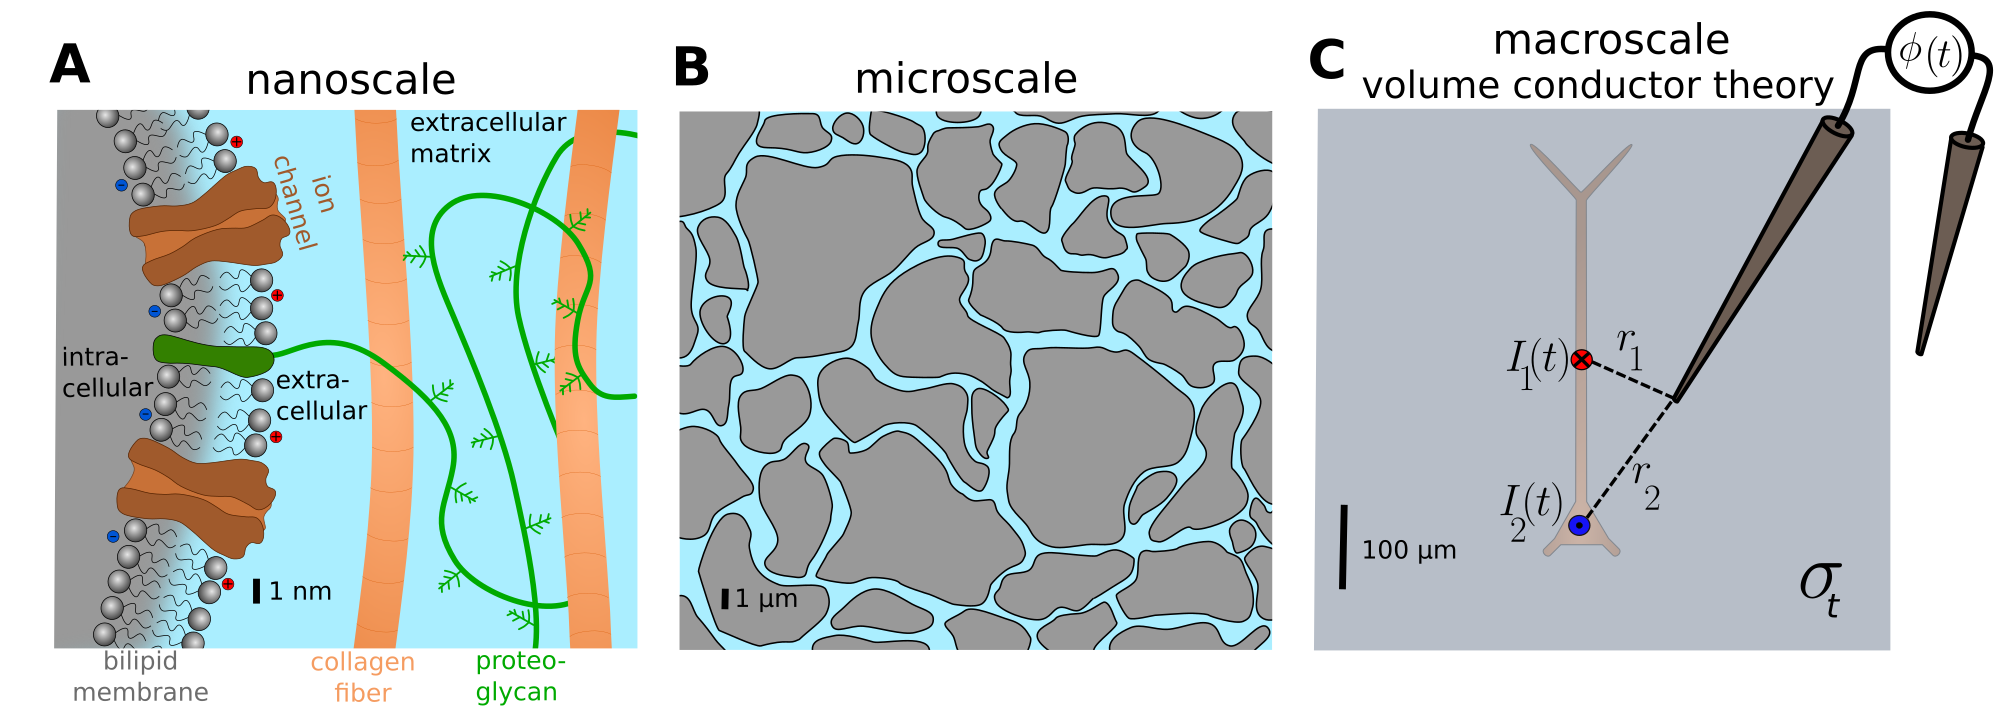
\includegraphics[width=1.0\textwidth]{Figures/VC/ecs_scales_three_levels.png}
\end{center}
\caption{\textbf{Extracellular space on different spatial scales.} (A) Nanometer scale. (B) Micrometer scale. (C) Millimeter scale. 
Panel C is the level where we apply VC theory
\tvnnote{Denne figuren er ogsaa i VC, men passer kanskje best her?}
\ghnote{Er mum-scale-baren i B litt liten? Er det rimelig at alle strukturer har diameter stoerre enn 1 mum? Har lest at typisk avstand ml. to celler er 60 nm, men her ser det mer ut som 1 mum.}
}
\label{fig:Basics:ECS_scales_3levels}
\end{figure}

%%%%%%%%%%%%%%%%%%%%%%%%%%%%%%%%%%%%%%%%%%%%%%%%%
\section{\blue{Electric currents}}
\label{sec:Basics:Current} \index{Electric current}
%As was argued in the previous subsection, we do not (and can not) study a macroscopic system by keeping track of individual particles or charges, but rather in the average movement of particles or charge on a larger spatial scale.
%Although \tvntxt{charges and forces, as we have discussed up until now,} establishes the fundamental origin for electric interactions, there is a fairly long way to go from these equations (e.g., \fref{eq:Basics:CoulombFN}) to the understanding of electric phenomena in a macroscopic system such as the brain. When describing a macroscopic system, we are usually not interested in the microscopic interactions between a small number of charges, but rather the joint interactions of a very, very large number of charges. It is then not feasible to keep record of the position of each individual charge, but rather to work with continuous variables defined on a larger spatial scale, such as charge densities, $\rho$ (with units \si{\coulomb\per\cubic\metre}), or ion concentrations, $c_k$ (with units millimolar ($1\, \si{\milli\molar} = 1 \,\si{\mole\per\cubic\metre} = 6.02\times10^{23}$ particles per \si{\cubic\metre})). The movement of particles of a given species $k$ is then quantified in terms of a particle flux, $J_k$, with units \si{\mole\per\second}, and the movement of charge is quantified in terms of an electric current, $I$, with units ampere (\si{\ampere} = \si{\coulomb\per\second}).
%The movement of particles of a given species $k$ is then quantified in terms of a particle flux, $J_k$, with units \si{\mole\per\second}, and the movement of charge is quantified in terms of an electric current, $I$, with units ampere (\si{\ampere} = \si{\coulomb\per\second}). 
An electric current represents a net movement of charge. An important concept that we will return to many times in this book is that of {\it current conservation}\index{current conservation}, i.e., the requirement that the the sum of currents into a finite volume of space must be zero. Current conservation is a slightly less fundamental version of the charge conservation discussed earlier in this chapter (\fref{sec:Basics:Charge}). 

When charge conservation is combined with electroneutrality (\fref{sec:Basics:Debye}), current conservation automatically follows: The net amount for charge entering a finite volume must me zero, because otherwise charge would pile up there and violate electroneutrality. In certain cases, electroneutrality is not fulfilled. For example, charge can pile up locally on both sides of circuit elements known as capacitors. However, since charge is conserved, the accumulated charge can be released as a current at a later time. \ghtxt{Furthermore, it is customary to describe also the charge accumulation process itself in terms of a \textit{capacitive current}, which allows the concept of current conservation to be applied also to the charging of a capacitor. }

There exist various kinds of electric currents, differing in terms of what drives them, and the content of the last paragraph will hopefully become more clear when we below introduce the three kinds of currents that are most important for the topic of this book. These are conductive currents (\fref{sec:Basics:ConductiveCurrent}), capacitive currents (\fref{sec:Basics:CapacitiveCurrent}) and diffusive currents (\fref{sec:Basics:DiffusiveCurrent}). We also briefly comment on inductive and advective currents (\fref{sec:Basics:OtherCurrents}), although we will assume that these are of negligible importance for the brain dynamics that we study in this book. 


\subsection{\blue{Conductive currents}}
\label{sec:Basics:ConductiveCurrent}
\index{Conductive current}
A conductive material \index{Conductive medium} is one through which charges can move freely when they are exposed to an electric field. The field-driven motion of charges can be quantified in terms of a conductive current, defined as the amount of charge that moves through some reference cross-section of the material area per second.

In electric circuits composed of metallic wires and various circuit elements, currents are essentially in 1D, running in the directions defined by the circuitry. The reference cross-section area is then typically taken to be that of "the whole wire" or "the whole circuit element". We then do not have to worry about the reference cross-section area, but can simply define the total current at each part of the circuit. A simple example is shown in \fref{fig:Basics:Currents}A, where a current passes through a wire with a resistor. The current is then given by Ohm's law:
\begin{equation}
I = - \frac{\Delta V}{R},
\label{eq:Basics:Ohm_R}
\end{equation}
where $\Delta V = V_B-V_A$ is the voltage difference across the resistor, and $R$ (units Ohm (\si{\ohm})) its resistance. Here, the wire itself is assumed to have a zero resistance, so that the entire resistance in the system, and the entire voltage drop, is that over the resistor. To describe this system, we only need to consider the potential at two locations, $A$ and $B$, representing the two sides of the resistor.

\begin{figure}[!ht]
\begin{center}
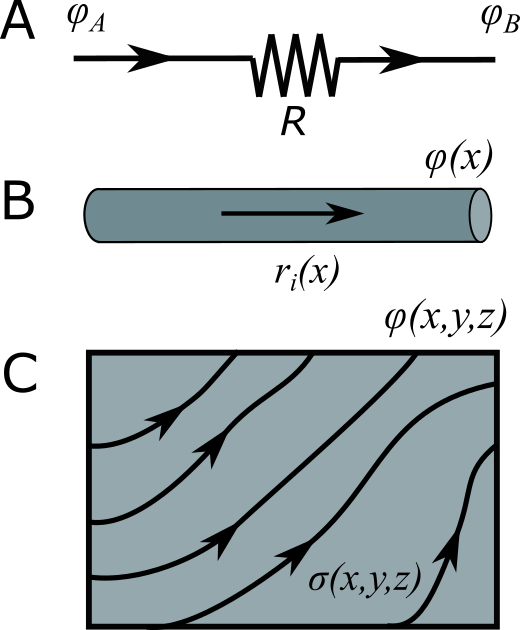
\includegraphics[width=0.6\textwidth]{Figures/Basics/Currents.png}
\end{center}
\caption{{\bf Ohms law for currents and current densities.} {\bf (A)} Current through wire and resistor with resistance $R$ (\si{\ohm}): $I = (V_B-V_A)/R$. {\bf (B)} Current in wire with specific axial resistance per unit length $r_\text{a}$ (\si{\ohm\per\metre}).  $I=- (1/r_\text{a}) dV/dx$. {\bf (C)} Current density (\si{\ampere\per\square\metre}) for current passing through a volume conductor with conductivity $\sigma$ (\si{\siemens\metre}): ${\bf i} = \sigma {\bf E} = - \sigma {\bf \nabla} V$. Current paths will depend on $\sigma(x,y,z)$ which generally can vary with position. Note that in all three cases we have current conservation, meaning that for an arbitrarily defined closed volume, the exact same amount of current will enter and exit the volume.
}
\label{fig:Basics:Currents}
\end{figure}
In reality, the resistance of the wire is not strictly zero, but for most standard electrical circuits it is an excellent approximation. However, in some applications, for example if the wire is very long and thin, or if it is made of a less conductive material, it may be necessary to treat it as a continuous resistor. If we define the specific axial resistance per unit length $r_\text{a}$ (units \si{\ohm\per\metre}), Ohm's law becomes:

\begin{equation}
I = - \frac{1}{r_\text{a}}\frac{dV}{dx},
\label{eq:Basics:Ohm_r}
\end{equation}
where $r_\text{a}=r_\text{a}(x)$ may in principle vary along the wire (\fref{fig:Basics:Currents}B). With \fref{eq:Basics:Ohm_r}, the potential $V(x)$ will vary gradually along the wire. If $r_\text{a}$ is constant along the wire, and the wire has length $L$, it is related to the resistance of the total wire through $r_\text{a}=R/L$. As we shall see in \fref{sec:Neuron:morphology}, conductive currents running axially through neural dendrites and axons are typically modeled in this manner. 

The examples above were both 1D in the sense that the current was restricted to run exclusively in the direction defined by the wire. In a 3D volume, such as for example brain tissue, currents may run in all spatial directions (\fref{fig:Basics:Currents}C). It is then convenient to describe them in terms of a current density, ${\bf i}$ (units \si{\ampere\per\square\metre}), a vector that defines the current per unit cross section area and its spatial direction. The current density\index{Current density} can be defined in all points in 3D space. The conductive properties of a material can be specified either through its resistivity $r$ (units \si{\ohm\metre}), or its inverse, the conductivity $\sigma$ (units \si{\siemens\per\metre}), both being material properties. We will here use the latter convention, and with that, Ohm's law takes the form:
\begin{equation}
{\bf i} = - \sigma {\bf \nabla} V,
\label{eq:Basics:Ohm_3D_phi}
\end{equation}
%
or, equivalently (cf. \fref{eq:Basics:EV}):
\begin{equation}
{\bf i} = \sigma {\bf E}.
\label{eq:Basics:Ohm_general}
\end{equation}
Note that in general the conductivity can be inhomogeneous, that is, position-dependent, so that $\sigma \rightarrow\sigma(x,y,z)$.

\subsubsection{\blue{A note on Ohm's law}}
\label{sec:Basics:Note}
It is important to remember that Ohm's law (\fref{eq:Basics:Ohm_general}) represents the average movement of charge on larger spatial scales, and does not apply for movement of individual charges on the nanometer scale. If we compare it with the physical foundations for electric interactions, it is easy to get confused, so let us dive into that confusion and try to clear it up. According to \fref{eq:Basics:E}, an electric field acts on a reference charge $q$ by a constant force, and should according to Newton's law (${\bf F} = m{\bf a}$) give it a constant acceleration in the field-direction. Conversely, \fref{eq:Basics:Ohm_general} states that ${\bf E}$ gives rise, not to a constant acceleration of charges, but rather a constant current, i.e., a constant average \textit{velocity} of charges.

The reason for the discrepancy between the single charge (constant acceleration) and many-charge (constant velocity) scales is that the constant acceleration (eq. \ref{eq:Basics:E}) of our single protagonist charge $q$ will go on for only a tiny time period \ghtxt{(much smaller than the charge relaxation time)} before it will bump into some other particle and be scattered out in some random direction. After the scattering event, the acceleration will start "from scratch", and go on until the next collision takes place, and so forth.  \gen{Dette bildet er litt enklere aa forstaa for noytrale partikler som ikke paavirkes av langtrekkende krefter.} \ghnote{Hva mener du her? Vi snakker om Ohms lov. Noyetrale partikler har diplomatisk immunitet.} Whereas the scattering events will tend to make the motion of $q$ a random walk (which should give it a zero average velocity in any preferred direction), the small periods of acceleration between collisions will at average give $q$ a net drift velocity in the field direction. As the same will happen for all other charges present, there will be a net drift of charge in the field direction. The current density given by \fref{eq:Basics:Ohm_general} is therefore often referred to as the \textit{drift current density}\index{Drift current}. Admittedly, the explanation that we proposed here was somewhat hand-waving, and the fact that we get the linear relationship between the current and the electric potential/field in \fref{eq:Basics:Ohm_general} is constitutive, meaning that it is observed experimentally rather than derived from first physical principles. It is found to be a good approximation for many mediums under many conditions, and an excellent approximation for brain tissue \cite**{nicholson1975,Nunez2006,Logothetis2007,Miceli2017}.

\ghtxt{The maximum drift velocity of electrons in copper wires carrying household electricity is in the order of $10^{-4}$-- $10^{-3}$\si{\metre\per\second}, while the drift velocity of ions for large-scale currents in brain tissue is only in the order of $10^{-9}$--$10^{-8}$ \si{\metre\per\second}. Importantly, this, perhaps counterintuitively slow drift velocity should not be confused with the "speed of electricity". When turning on a light switch, and electric field will spread throughout the wire with a speed close to the speed of light, and will just take about a nanosecond to obtain a drift velocity of electrons throughout the entire wire. }

\gen{Igjen: Er denne tiden den samme som charge-relaxation time til elektronoytralitet?} \ghnote{Nei, det er i hvert fall ikke aapenbart. Jeg tok bort disse referansene til charge-relaxation time. I dette siste tilfellet er svaret mitt "kanskje". Det finnes to tidsskalaer:  I Drude-formelen kalles tiden mellom to kollisjoner for "relaxation time". Denne er mye kortere enn "charge relaxation time". Ohms lov gjelder kun for mye stoerre tidsskalaer enn "relaxation time". Utledningen av "charge relaxation time" antar imidlertid at Ohms lov gir oss stroemmen. Med andre ord faar man tro at Ohms lov faar sin gyldighet et sted mellom relaxation time og charge relaxation time. Har ikke funnet noen klare formuleringer om sammenhengen ml de to, men det burde det sikkert finnes et sted. Jeg antar at naar man trykker paa bryteren, saa kommer stroemmen like raskt som Ohms lov begynner aa gjelde. Dette skjer altsaa et sted mellom relaxation time og charge relaxation time. Jeg heller mot at sistnevnte gir den beste pekepinnen, men vi trenger nok ikke aa uttale oss om saken.}

\ghnote{La til siste avsnitt, fordi det er artig aa bli forbloeffet over at drifthastigheten er saa lav. Ser det ok ut? Litt usikker paa aa angi tall for drifthastighet i tissue. Kanskje burde vi bare skrive at den nok er mye lavere enn i en kobberkabel, noe jeg synes folk flest burde kunne ta for god fisk. Brukte her regnestykket: ${\bf u}_\text{drift} = \sigma_\text{t} E/(-e[q]n_A)$, og antok typiske verdier, $\sigma_\text{t} = 0.2 \si{\siemens\per\metre}$, $E\sim 1 \si{\volt\per\metre}$ (typisk DC potensial paa 1 mV over 1 mm mellom topp og bunn av cortex), samt konsentrasjon av ladningsbaerere paa $[q] \sim 300 \si{\milli\molar}$. Det ga meg 6 nm/s, om jeg husker riktig, men drift kan sikkert vaere stoerre enn dette paa mindre skala etc. Drifthastigheten for Na-stroem over membranen under AP er ca. 1 mm/s. Tipper at dette vil vaere maksimalverdi i hjernen. Gudene vet, men har enn saa lenge ikke nevnt det i noen av sine publikasjoner.}
\gen{Nei, gudene er ofte slappe med aa publisere (har vel egentlig ikke publisert noe saerlig paa flere tusen aar). Synes det er kult aa ta med, men kanskje vi kan si noe om drift velocity i kobberledningen til en vanlig lampe (hvis mulig), siden vi er kvalitative og ikke alle har et forhold til hva 20 Ampere er?} \ghnote{Gikk for maxiumum household - tenker at 20 A er maksimalverdi. Lampa er ca. 0.2 A, og gudene vet hvor tykk traaden er.}


%${\bf u}_\text{drift} = \sigma_\text{t} E/(-e[q]n_A)$. Here, $e$ is the unit charge and $N_A$ Avogadros number. If we use typical values for brain tissue, assuming a conductivity $\sigma_\text{t} = 0.2 \si{\siemens\per\metre}$, a field strength $E\sim 1 \si{\volt\per\metre}$ a concentration of charge carriers $[q] \sim 300 \si{\milli\molar}$, we get an estimate $v_{drift} \sim 10 \si{\nano\metre\per\second}$. This is a very small velocity, so our main candidate will be the bulk flow (iii). Since the bulk solution on the brain is electroneutral, advective bulk flow does not carry any net charge. However, it does carry positive and negative ions in a given direction, and a magnetic field bend the oppositely charged ions in opposite directions. The maximal blood flow velocity through arteries has been estimated to be ${\bf u}_\text{bulk} \sim 1 \,\si{\metre\per\second}$ \cite**{bishop1986}, and we may take this s an upper limit for a the bulk flow velocity in the brain. 


\subsection{\blue{Capacitive currents}}
\label{sec:Basics:CapacitiveCurrent}
\index{Capacitive current}
A common element in electrical circuits is the capacitor. Capacitors are devices that can store electric charge. The simplest form of a capacitor, a parallel plate capacitor, consists of two electrical metallic plates or surfaces separated by an insulating (dielectric) medium\index{Dielectric medium}. By definition, a dielectric medium is one where charges are bound to stay in confined regions of space. An electric field will only slightly shift their average equilibrium positions, causing a polarization of the material. 

A parallel plate capacitor can separate a charge $q$ on one plate from a charge $-q$ on the other plate, to obtain a voltage difference:
\begin{equation}
V = \frac{q}{C},
\label{eq:Basics:Vcap}
\end{equation}
where $C$ (units farad (\si{\farad} = \si{\coulomb\per\volt})) is the capacitance.

To understand how a capacitor works, consider the illustration in \fref{fig:Basics:Capacitor}, where a conductive current $I_\text{in}$ enters the capacitor from the left, and a conductive current $I_\text{out}$ leaves to the right. Whereas $I_\text{in}$ and $I_\text{out}$ are mediated by charges moving freely through cables, no charges actually move across the capacitor itself. Instead, $I_\text{in}$ leads to an accumulation of charge $dq/dt$ on the left metal plate of the capacitor. This, in turn, evokes an electric field across its dielectric core, which drives positive charges away from the rightmost metal plate, charging it negatively $-dq/dt$. The temporal rate of change of the electric field across the dielectric medium can be described in terms of a \textit{capacitive current} defined by:
\begin{equation}
I_\text{cap} = \frac{dq}{dt} = C\frac{dV}{dt},
\label{eq:Basics:Icap}
\end{equation}
Although $I_\text{cap}$ differs from conductive currents in the sense that it does not involve free transfer of charge through a medium, it has the same units (A), and ensures currents continuity so that $I_\text{in} = I_\text{cap} = I_\text{out}$. 

\begin{figure}[!ht]
\begin{center}
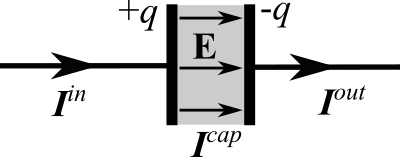
\includegraphics[width=0.6\textwidth]{Figures/Basics/Capacitor.png}
\end{center}
\caption{{\bf Capacitor}.  In the simplest form, a capacitor consists of two electrical metallic plates or surfaces separated by an insulating (dielectric) medium. Charges $q$ and $-q$ on the metal plate generate an electric field $E$ in the dielectric medium, or a potential difference, $V = Ed$ where $d$ is the distance between the metal plates. We skipped the vector notation on $E$ since the field direction is implicit.
}
\label{fig:Basics:Capacitor}
\end{figure}

The capacitive current was introduced here because neural membranes have capacitive properties, which causes the neural membrane potential to change when currents pass through the membrane. It is customary to express the capacitive membrane current in terms of a current density, i.e., as current per membrane area:

\begin{equation}
i_\text{cap} = c_m\frac{dV_m}{dt},
\label{eq:Basics:Icap_mem}
\end{equation}
where $c_\text{m}$ (units \si{\farad\per\square\metre}) is the capacitance per unit membrane area. \ghtxt{\sout{In this case, the current density is in 1D and in the direction normal to the membrane.}}
\gen{Litt forvirrende: Current density er jo per areal, men stroemmen er rettet kun i 1 retning.}
\ghnote{Hvorfor er det forvirrende? Blir det bedre om jeg stryker siste setning?}



\subsection{\blue{Diffusive currents}}
\label{sec:Basics:DiffusiveCurrent}
\index{Diffusion} \index{Diffusive current}
The charge carriers in the brain are ions floating around in the saline solutions that fill up the intra- and extracellular spaces. Ions in salt water will, like electrons in a metal conductor, be accelerated by the presence of an electric field, and will thus carry conductive currents in accordance to Ohm's law (\fref{eq:Basics:Ohm_general}). In addition to movement propelled by the electric field, ions in water may also move due to diffusion. If the concentration ($c_k$) of an ion species $k$ varies with position, diffusion will tend to drive ions towards regions with low concentration, and since ions carry electric charge, this movement amounts to an electric current that comes in addition to the conductive current. 

The electrodiffusive \index{Electrodiffusion} nature of ionic motion is described by the Nernst-Planck equation\index{Nernst-Planck equation},
\begin{equation}
{\bf j}_k = - D_k {\bf \nabla} c_{k} - \frac{D_k z_k c_k}{\psi} {\bf \nabla} V,
\label{eq:Basics:JNP}
\end{equation}
which determines the flux density, ${\bf j}_k$ (units \si{\mole\per\square\metre\per\second}) of an ion species $k$. The valency, $z_{k}$, is a unit-less number that denotes the number of unit charges associated with a single ion of species $k$. The factor $\psi=RT/F$ (units \si{\volt}) is defined by the gas constant ($R = 8.314 \, \si{\joule\per\mole\per\kelvin}$), Faraday's constant ($F = 96458.3\, \si{coulomb\per\mole}$), and the temperature ($T$ with units \si{\kelvin}).

The first term on the right hand side of \fref{eq:Basics:JNP} is Fick's law for diffusion, and states that the diffusive flux of ion species $k$ is proportional to the diffusion constant ${D}_k$ (units \si{\square\metre\per\second}) times the concentration gradient ${\bf \nabla} c_{k}$. ${D}_k$ is a property of the medium that the ion diffuses through, and determines how "easy" it is for the ion $k$ to move through the medium. The second term on the right hand side of eq. \ref{eq:Basics:JNP} accounts for ionic drift due to the electric field. 
\gex{The derivation of this second term builds on two assumptions.The first is that the drift velocity 
${\bf u}_k$ of ion $k$ when acted upon by a force ${\bf F}$ is given by
\begin{equation}
{\bf u}_k = \mu_k {\bf F}, 
\label{eq:Basics:mobility}
\end{equation}
where $\mu_k$ is the mobility\index{mobility} of ion $k$. The second assumption is that the mobility and diffusion constant is related via the so-called  Einstein relation\index{Einstein relation}: 
\begin{equation}
D_k = \mu_k \psi, 
\label{eq:Basics:EinsteinRelation}
\end{equation}
The Einstein relation does not apply generally, but is valid for dilute saline solutions, such as the saline solution in the brain \cite**{Grodzinsky2011}. }
\gen{Litt usikker paa valg av symbol for drift velocity. Er $u$ OK?}

Faraday's constant is defined as the charge per mole ($6.02\times10^{23}$) of unit charges. A flux density ${\bf j}_k$ can thus be converted to a current density by multiplying it with $Fz_k$. A salt-water solution is composed of several ions, and to obtain the net electric current, we can sum over the contributions from all of them to obtain the total current density:
\begin{equation}
{\bf i} = \sum_k z_k F {\bf j}_k = -\sum_k{F z_k {D_k}{\bf \nabla} c_{k}} - F\sum_{k} \frac{{D_k} z_{k}^2}{\psi}c_{k} {\bf \nabla}{V}.
\label{eq:Basics:iNP}
\end{equation}
The last term on the right hand side is the drift current density,
\begin{equation}
{\bf i}_\text{drift} = - F\sum_{k} \frac{{D_k} z_{k}^2}{\psi}c_{k} {\bf \nabla}{V} = - \sigma {\bf \nabla}{V}.
\label{eq:Basics:idrift}
\end{equation}
As we indicated with the last equality, the drift current density is the same as the Ohmic current that we defined in eq. \ref{eq:Basics:Ohm_3D_phi}, which means that we can identify the conductivity $\sigma$ of a salt-water solution as:
\begin{equation}
\sigma = \frac{F}{\psi}\sum_{k} {D}_k z_{k}^2 c_{k},
\label{eq:Basics:sigma_conc}
\end{equation}

The first term on the right hand side of \fref{eq:Basics:iNP} is the diffusive current density,
\begin{equation}
{\bf i}_\text{diff}  = -\sum_k{F z_k {D_k}{\bf \nabla} c_{k}}.
\label{eq:Basics:idiff}
\end{equation}
Hence, in a conductive medium that contains concentration gradients, the total current is not purely Ohmic, but can contain an additional contribution from ionic diffusion. 

In many cases, the total current will be dominated by the drift component, and although it is possible that ionic diffusion sometimes plays a role (see \fref{chap:Schemes}), it is common to assume that the diffusive component is negligible when modeling extracellular currents in the brain. The diffusive current does, however, play an important role for currents across neuronal membranes.

\subsection{\blue{Other currents}}
\label{sec:Basics:OtherCurrents}
Generally, currents additional to those defined above may arise due to advection or magnetic induction. An advective current\index{Advective current},
\begin{equation}
{\bf i}_\text{adv} = F \rho {\bf u},
\label{VC:eq:iadv}
\end{equation}
arises in a bulk solution if the solution has a charge density $\rho$ that it drags along with it due to a bulk flow with velocity ${\bf u}$. However, as we argued in \fref{sec:Basics:Debye}, the saline solution in the brain is practically electroneutral ($\rho \simeq 0$), and the advective current is \gex{thus} expectedly negligible. A more thorough argument for this was given in \citeasnoun**{Gratiy2017}.

As we briefly touched upon earlier, charges may also be accelerated by changes in a magnetic field ${\bf B}$, which gives rise to so-called inductive current proportional to $\partial {\bf B}/\partial t$. However, in the brain, such inductive currents caused by the magnetic field are assumed to be of negligible importance \cite**{Ranck1963,plonsey1967,Bossetti2008} (more about this in \fref{sec:Basics:Maxwell}).


%%%%%%%%%%%%%%%%%%%%%%%%%%%%%%%%%%%%%%%%%%%%%%
\section{\blue{Electric currents in the brain}}
\label{sec:Basics:braincurrents}
The main focus in this book is on modeling and interpreting extracellular potentials in the brain. As we indicated earlier, an expression for the extracellular potentials originating from neural activity can be derived from the principle of current conservation. Let us therefore start this endeavor by defining the types of currents that are relevant in different components of brain tissue.

Having introduced different kinds of currents in \fref{sec:Basics:Current}, we can now summarize the role they play within a brain-specific context. It is useful to make a distinction between currents existing in one of three different mediums, being either:
\begin{itemize}
\item intracellular currents 
\item extracellular currents 
\item transmembrane currents  
\end{itemize}
\gen{Tok bort punktum og stor bokstav}

Among these three, the membrane currents are the odd ones out. A bit cartoonishly, we may think of the cellular membrane as an insulator with small holes. The insulating properties give the membrane the ability to separate charges in the conductive solution on the cellular outside from charges in the conductive solution the cellular inside. Nonzero charge densities are then stored in so-called \textit{Debye-layers}\index{Debye-layer} on the in- and outside of the membrane, equivalent to how charges are stored on the metal plates in a parallel plate capacitor (cf. \fref{fig:Basics:Capacitor}). 

This charge-storage process can be described in terms of a capacitive current as defined in \fref{eq:Basics:Icap_mem}, which causes the membrane potential to vary with time. The holes represent various kinds of ion channels, which are conductive pores in the membrane allowing ions to pass through. Ionic currents through ion channels come in addition to the capacitive current. The capacitive and conductive membrane currents are both essentially one-dimensional and perpendicular to the membrane. They depend both on voltage- and ion concentration differences between the inside and outside of the membrane, and are thus electrodiffusive in their nature, cf. \fref{eq:Basics:iNP}, but in one dimension, so that ${\bf \nabla} \rightarrow d/dx$.

The intra- and extracellular currents are generally three-dimensional electrodiffusive volume currents (cf. \fref{eq:Basics:iNP}) through the conductive saline solutions that fill up the intra- and extracellular spaces. However, as concentration gradients within the \gex{intra-} and extracellular spaces typically are much smaller than those across membranes, it is common to neglect the diffusive component and approximate the intra- and extracellular currents as being purely conductive (cf. \fref{eq:Basics:Ohm_3D_phi}). An illustration of the involved currents in a small piece of tissue is given in \fref{fig:Basics:Twostep}A. As indicated there, currents travel in loops, so that the intracellular and extracellular currents are coupled through the transmembrane currents at the cellular boundary. 

For intracellular currents it is common to make the further simplification that they are well approximated as being in 1D (cf. \fref{eq:Basics:Ohm_r}). 
\gen{Antagelsen er vel egentlig at stroemmen kun gaar i 1 retning. Kan vi vaere med presise?} 
This is motivated by the morphological structure of neurons, which fairly accurately can be represented as branching cables of varying diameter (\fref{fig:Basics:Twostep}B).

\begin{figure}[!ht]
\begin{center}
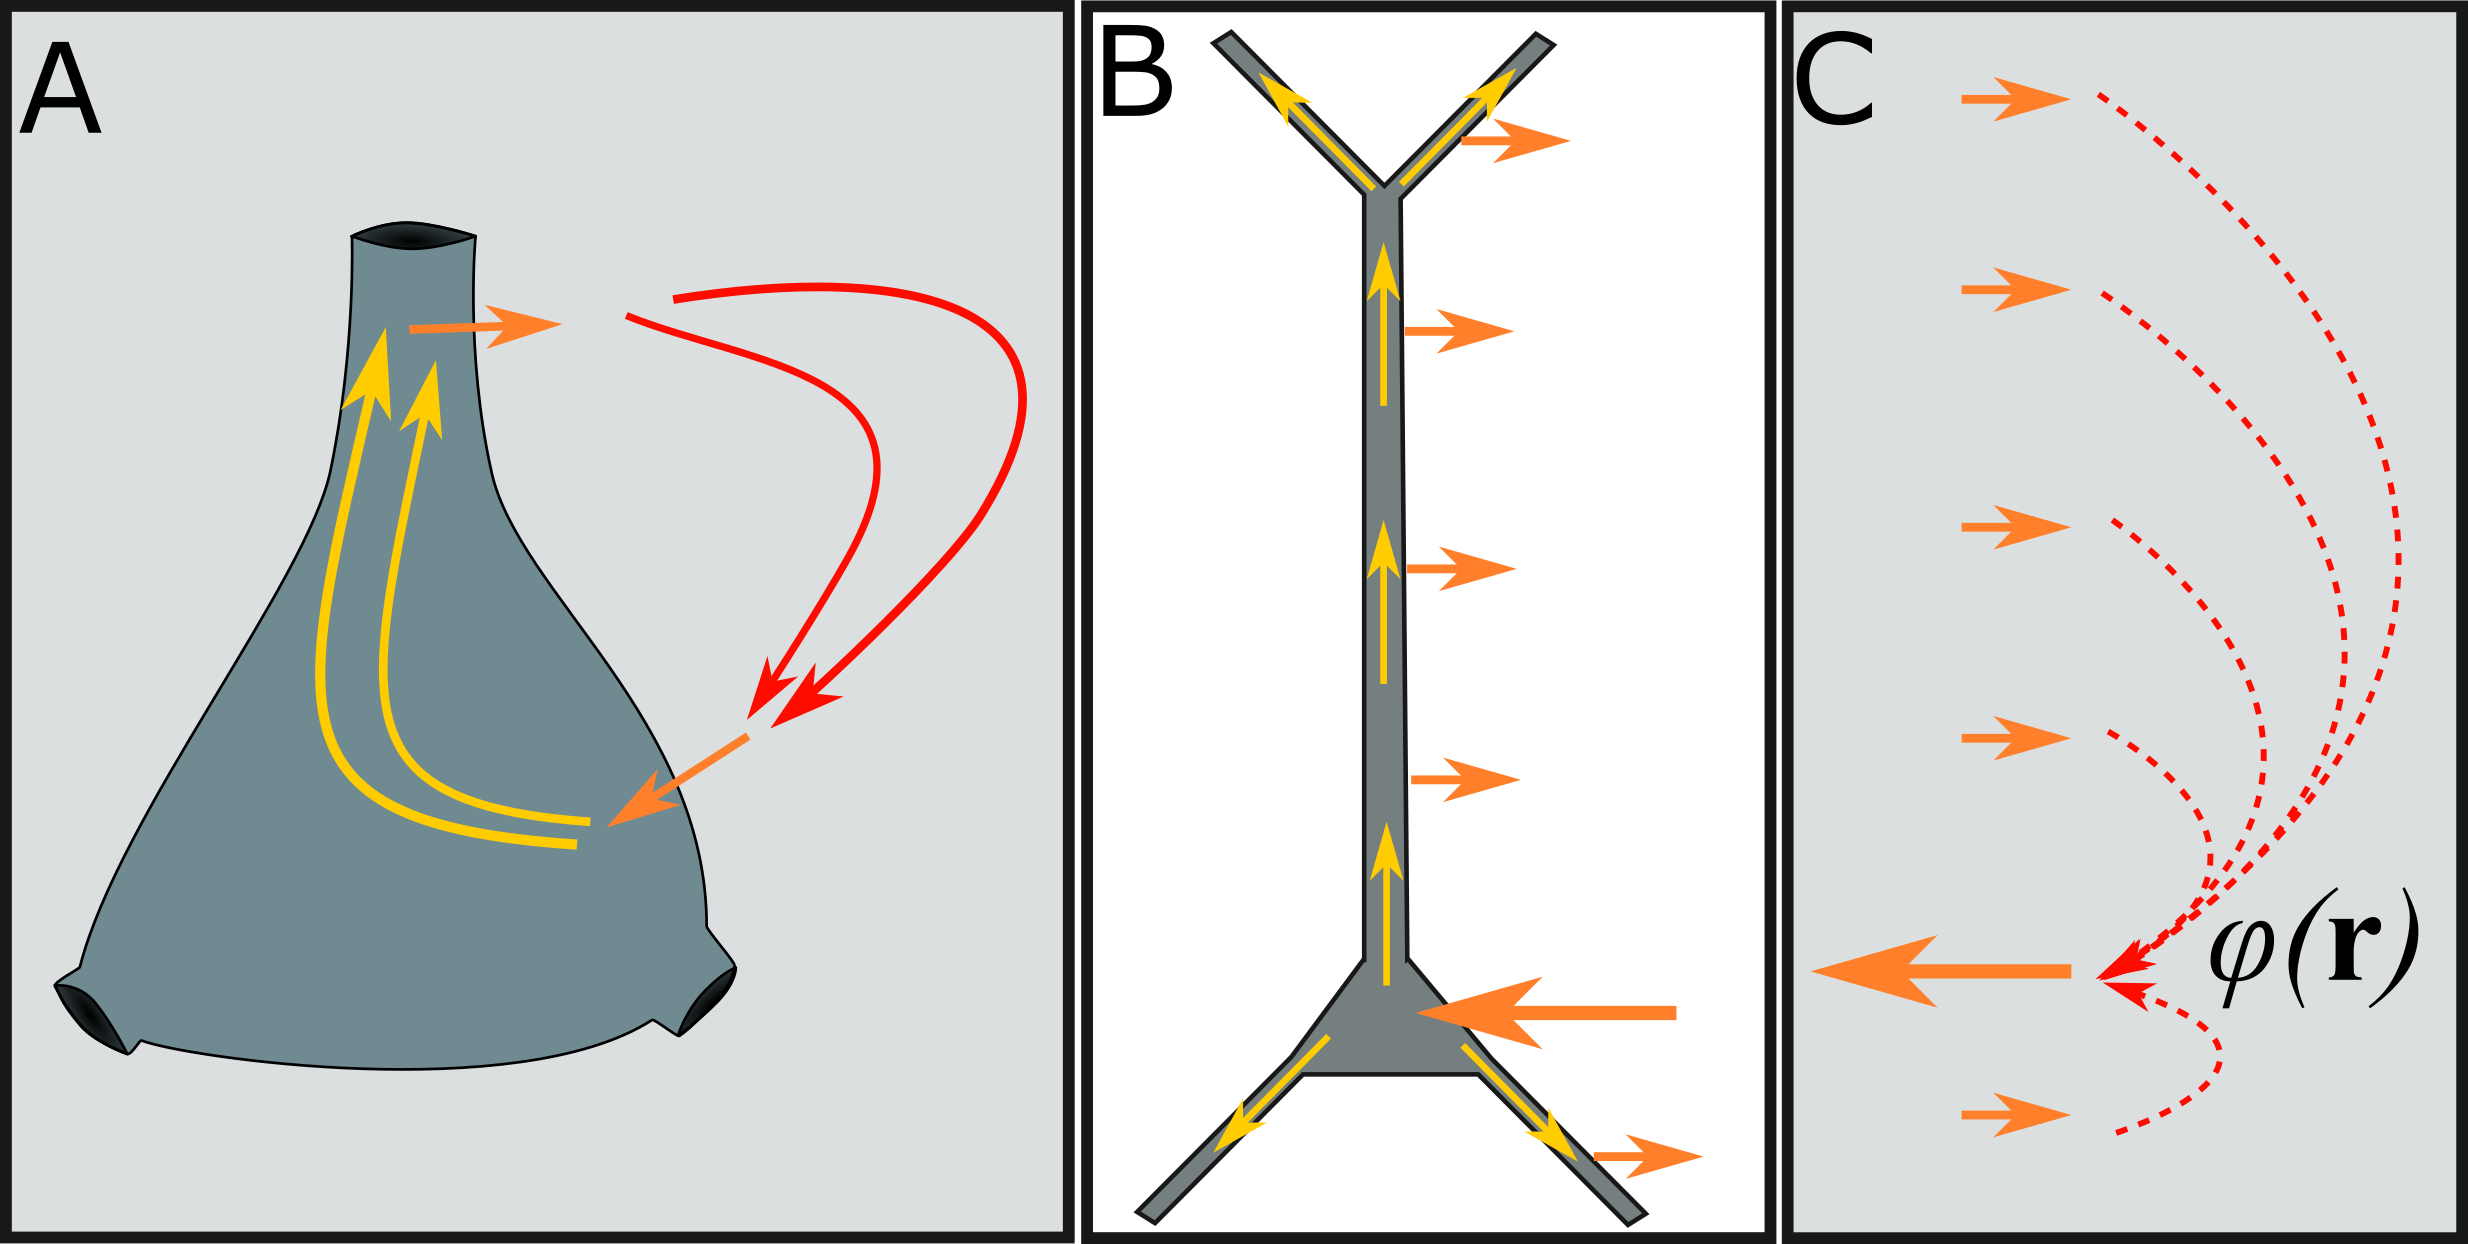
\includegraphics[width=1.0\textwidth]{Figures/Basics/Twostep.png}
\end{center}
\caption{{\bf Currents in brain tissue}. {\bf(A)} Illustration of currents involved in the brain, with intracellular volume currents (yellow), extracellular volume currents (red), and transmembrane currents (orange). Currents travel in closed loops. The entire space will be filled with currents, and only a few paths was included in the illustration. {\bf(B)} A standard modeling strategy is to compute the intracellular and transmembrane currents on a framework independent of the extracellular dynamics. The neuron is approximated as a branching cable, and intracellular currents are one-dimensional along the cable, whereas transmembrane currents are perpendicular to the cable and distributed over the cable. {\bf(C)} The transmembrane currents computed in the framework {\bf(B)} can be used as output sources and sinks to the extracellular space, and can be used to compute the extracellular potential $V({\bf r})$. This will be the potential that is "needed" to complete all current loops, a few of which are illustrated with red, dashed arrows.
\tvnnote{Kanskje holde oss til "to-kompartment" versjon av cella i B, for enkelthets skyld? Altsaa én intracellulaer stroem, og to membran-stroemmer, samt symmetriske volum-stroemmer paa begge sider av cella. Kan ogsaa kanskje tegne inn noen
stiplede firkanter som representerer "volum", for aa gjoere et poeng av at volum uten kilder har stroem, men like mye ut som inn, mens membranstroemmer kan sees paa som kilder/sluk. Dette kunne vaert fint for diskusjon rundt ligning (2.27) i "Neurons as current sources".} \ghnote{Ok, skal.}
}
\label{fig:Basics:Twostep}
\end{figure}


\section{\blue{Jumping up in spatial scale 2: From a mishmash of entangled neurites to smooth neural tissue}}
\label{sec:Basics:ECSpot}
Brain tissue is a dense mishmash of neurites and other cellular structures, where about 80\% of the volume is occupied by cells, and about 20\% is the highly tortuous\index{Tortuosity} extracellular space. The diameter of a typical neurite is on the order of 1 \si{\micro\metre}, and the extracellular space between cellular membranes is typically as narrow as 40-60 \si{\nano\metre} \cite**{Sykova2008}. Due to the principle of current conservation, a transmembrane current (defined in the previous section) at some location must "continue" as an extracellular current and somehow make its way through the tissue mishmash. Current conservation in tissue is the fundamental principle that we use for modeling extracellular potentials.

Locally, electric currents in the narrow confines of extracellular space may have a free passage through the extracellular saline solution only in certain spatial directions, whereas passage in other directions is blocked by cellular membranes with a much higher resistance than saline. Hence, a micrometer-precice insight into the pathways taken by extracellular currents requires knowledge of the highly inhomogeneous microstructure of the tissue. Although small volumes of tissue can be partially reconstructed {\it ex vivo} using techniques like scanning electron microscopy, the overall microstructure is almost always unknown, and even if it were known, including it in modeling or analysis of extracellular potentials would require prohibitively (in some cases impossibly) large computational resources. Keeping track of the exact microstructure of neural tissue is therefore practically impossible. Luckily, it is also for most purposes unnecessary. 

In \fref{sec:Basics:scale_jump1} we explained how we can jump from a nanometer-scale system description based on interactions between individual atoms and charges, to a description that is valid \gen{applicable?} 
on a larger spatial scale, based on continuous variables such as concentrations and currents. How coarse the spatial resolution must be for the continuum description to be applicable depends on how densely packed the medium is with the particle species that we are interested in. For the main ion species and electric currents in the saline solutions in the brain, a micrometer resolution is more than coarse enough for a continuum description to be warranted. 

When we want to consider extracellular currents through brain tissue, we need to make a second jump in scale, related to how densely packed the brain tissue is, not with ions and atoms, but with cellular structures. As we explained just above, tissue is highly inhomogeneous on the micrometer scale. However, on a coarser spatial scale of, say, some tens of micrometers, we may assume that the micro-scale inhomogeneities tend to average out \cite**{nicholson1975,Okada1994,Logothetis2007,Goto2010,Ness2015}. With a precision level of some tens of micrometers, we can then assume that an extracellular current experiences tissue as a smooth and continuous conductive medium with a constant conductivity (for more details, see \fref{chap:VC}-\fref{chap:Sigma}). In such a medium, we can calculate how such currents give rise to extracellular potentials by use of Ohm's law for volume conductors (\fref{eq:Basics:Ohm_3D_phi}). Electrodes used for measuring extracellular potentials typical have surface areas of at least a few square micrometers, and thus have a precision level in the same ballpark. \gen{Er dette riktig maate aa tenke paa? Hmmm...kanskje det?} The treatment of tissue as a continuous medium is discussed in more detail in \fref{chap:VC}-\fref{chap:Sigma}.

%\ghnote{Tok vek torbjorns crowd-analogi. Synes ikke at people blocking people er en god nok analogi for neurites blocking currents. Satser paa at dette er klart nok uten analogi.}
%As a loose analogy, we can consider a person moving through a dense crowd of people. On the scale of one meter, the crowd will appear highly inhomogeneous as certain directions are blocked by other people. However, on the scale of say ten meters, all directions might be approximately as easy to move in, and the crowd can seem roughly homogeneous. Something similar can be expected to happen with neural tissue, which appears highly inhomogeneous at the micrometer scale, but will typically appear quite homogeneous at a scale larger than ten micrometers or so. Therefore, for the purpose of modeling and analysing extracellular potentials, it is common to approximate neural tissue as a smooth continuous conducting medium, with a constant conductivity, where we can calculate extracellular potentials by use of Ohm's law for volume conductors (\fref{eq:Basics:Ohm_3D_phi}).  

%, and 
%Analogous to how it is impossible and unnecessary to keep track of individual atoms and charges, it is therefore in practice impossible and 
%The recording of an electric potential requires an electrode, and the spatial extension of the electrode determines the spatial resolution of the recording. For example, an electrode placed in the extracellular space of the brain will record the average potential taken over the interface (typically a metal surface or liquid junction) between the electrode and the extracellular fluid, which normally is at least 1~\si{\square\micro\metre}. When we speak of an electric field or potential, we generally mean the average of these quantities taken over a certain volume of interest. 
%We started this chapter on the spatial scale of a single atom (\fref{sec:Basics:Charge}). Single charge interactions, taking place on the spatial scale of the Debye-length ($\sim 1 \, \si{\nano\metre}$) and temporal scale of the charge-relaxation time ($\sim 1 \, \si{\nano\second}$), may be important for understanding detailed properties in cellular membranes. However, in this book we are interested in processes on the larger spatial scale where it is meaningful to work with continuous variables such as ion concentrations, charge densities, particle fluxes and electric currents (\fref{sec:Basics:Charge}). 
%The Na$^{+}$ concentration in the extracellular space of the brain is $\sim 150 \, \si{\milli\molar}$, which means that a volume of $1 \, \si{\cubic\nano\metre}$ of extracellular space then contains (on average) only $150\times 6.02\times10^{23}\times10^{-27} \approx 0.1$ Na$^{+}$ ions. A concentration is therefore not a very meaningful concept on a spatial scale as small as this. Continuous variables such as ion concentrations, charge densities, particle fluxes and electric currents, therefore imply a spatial resolution $\gg 1 \, \si{\nano\metre}$. When working on this scale, we do not need to be concerned with details of single charge interactions taking place on the nanometer and nanosecond timescale \cite**{Grodzinsky2011}.


\section{\blue{Extracellular potentials in the brain}}
\label{sec:Basics:ECSpot}
In the previous section, we argued that neural transmembrane currents will cause extracellular currents, and that we can use Ohm's law for a smooth volume conductor to calculate the corresponding extracellular potential. Below, we show how we from this can derive an expression for the relationship between extracellular potentials and transmembrane currents.

\subsection{\blue{Neurons as current sources}}
\label{sec:Basics:C}
\index{Current source density}
%Although potentials fundamentally are due to the distribution of charges on a nanometre scale, the shielding effects that we discussed in \fref{sec:Basics:Debye} allow us to predict a macroscopic (coarse-grained) extracellular potential from the constraint that there should be no charge accumulation anywhere in the extracellular space.
%, or equivalently, that there should be no net electric current entering or leaving any finite volume of tissue.
%\tvnnote{Siste del av setningen kan kanskje vaere litt forvirrende, mtp kilder og sluk osv? Kanskje ogsaa litt rart aa foerst anta makroskopisk volum, og saa si at det skal gjelde "any finite volume"?}
%\tvnnote{Alternativ: ... there should be no charge accumulation anywhere in the coarse-grained description of neural tissue. Charge accumulation on neural membranes still occurs, but this charge accumulation will always be in balance on the intra- and extracellular side,
%and the course-grained description by definition includes both these domains.}
%On the coarse-grained tissue scale ($\gg 1 \,\si{\cubic\micro\metre}$) \gex{($\sim$ 1 mm or larger?)} , a common starting point for computing extracellular potential is the requirement that all currents entering or leaving through neuronal membranes must be conserved and distributed in the extracellular space. 
To link the extracellular potentials to transmembrane currents, we start with considering a transmembrane current source, which we denote $C$.
\gex{This is a volume current density with units \si{\ampere\per\cubic\metre}), and is 
commonly referred to as the current source density (CSD).} This source will evoke a current density in the surrounding tissue, which we denote ${\bf i}_{\rm t}$.
\gen{Det at C representerer "transmembrane" currents i et 3D-kontinuum hvor membraner egentlig ikke eksisterer kan vaere forvirrende. Kan vi hjelpe leseren ytterligere her? Kanskje en figur med to paneler som viser stroemmer som kommer ut av en membran baade i "virkeligheten" og i 3D-kontinuum?}

When the tissue currents are due to the source $C$, current conservation can be expressed mathematically through the continuity equation \cite**{nicholson1975}:
\begin{equation}
{\bf \nabla} \cdot {\bf i}_\text{t} = -C,
\label{eq:Basics:continuity1}
\end{equation}
%where the source term, $C$ (with units \si{\ampere\per\cubic\metre}), is called the current source density (CSD). 
The source $C$ represents the transmembrane output current per tissue volume, and includes both the a capacitive component and a component due to ions crossing the membrane. 
%We have let ${\bf i}_\text{t}$ denote the density of current running extracellularly through brain tissue. 
%It does not include intracellular or transmembrane neural currents.
%\ghnote{Det er vel strengt tatt feil aa si at ${\bf i}_\text{t}$ trenger aa vaere ekstracellulaer. Kan vi si at ${\bf i}_\text{t}$ er all running through brain tissue that is not accounted for by the CSD?}

In a volume of space where there is no transmembrane currents ($C = 0$), \fref{eq:Basics:continuity1} reduces to ${\bf \nabla} \cdot {\bf i}_\text{t} = 0$. This tells us that the spatial rate of change of the current ${\bf i}_\text{t}$ is zero, which means that there will be no net tissue current entering or leaving such a volume. Importantly, this does not mean that the tissue current itself must be zero. Currents can still run \textit{through} the volume, as long as the amount of current entering equals the amount leaving. In a volume that \textit{does} receive transmembrane currents, \fref{eq:Basics:continuity1} tells us that the current outputted from the neuron into that volume ($C$) must be carried away from that volume as an extracellular tissue current. As we will show in \Fref{chap:VC}, this conservation law is the foundation for modeling extracellular potentials arising from neural activity.

Throughout most parts of this book, we shall approximate brain tissue as a \textit{linear} Ohmic conductor, an approximation that we will discuss in further detail below. This means that the tissue current densities are given by Ohm's law for volume conductors (\fref{eq:Basics:Ohm_3D_phi}). When this is inserted into \fref{eq:Basics:continuity1}, we obtain a relationship between the neuronal current sources and the extracellular potential:
\begin{equation}
{\bf \nabla} \cdot \left(\sigma_\text{t} {\bf \nabla} {V} \right) = -C,
\label{eq:Basics:continuity2}
\end{equation}
where we have used the index $t$ to denote that $\sigma_\text{t}$ is the \textit{tissue} conductivity. If $\sigma_\text{t}$ does not vary across space, \fref{eq:Basics:continuity2} simplifies to the often used form:
\begin{equation}
\sigma_\text{t} \nabla^2{V} = -C.
\label{eq:Basics:continuity3}
\end{equation}
\gen{$\sigma$ varierer jo generelt med retningen og det kan rimelig enkelt tas med i modellen (mest kompakt via en tensor. Det dekkes vel i VC-kapitlet, men kan kanskje ogsaa nevnes her?}


\subsection{\orange{The physical interpretation of extracellular potentials in the brain}}
\label{sec:Basics:interp_pot_brain}
\ghnote{Litt usikker paa misjonen til dette delkapittelet, fordi (1) jeg foeler dette gir meg svar paa noe jeg egentlig ikke lurte paa, og (2) fordi vi snakker om aksjonspotensialer og ekstracellulaere spikes, og foregriper begivenhetenes gang. Men jeg forstaar at kapittelet er en darling av Torbjorn, og kanskje det er et fint perspektiv aa ta med. Jeg har forsoekt meg paa en ny versjon jeg opplever som anelsen tydeligere. Ta en vurdering paa dette i neste moete. Nedenfor er min versjon (oeverst) og Torbjorns (under). Flyttet ogsaa Torbjorns figur hit, da jeg syntes den passet bedre inn her, enn lenger oppe, der vi fortsatt ikke hadde oppdaget nevronet.}

An electric potential is a measure of the energy needed to move a positive unit of charge from a reference point to a measurement point (\fref{sec:Basics:interp_pot_charge}). As an example that illustrates this interpretation of the potential, let us consider the situation where an electrode records the extracellular potential near a neuronal soma firing an action potential (\fref{fig:Basics:elec_circuit}). 

\begin{figure}[!ht]
\begin{center}
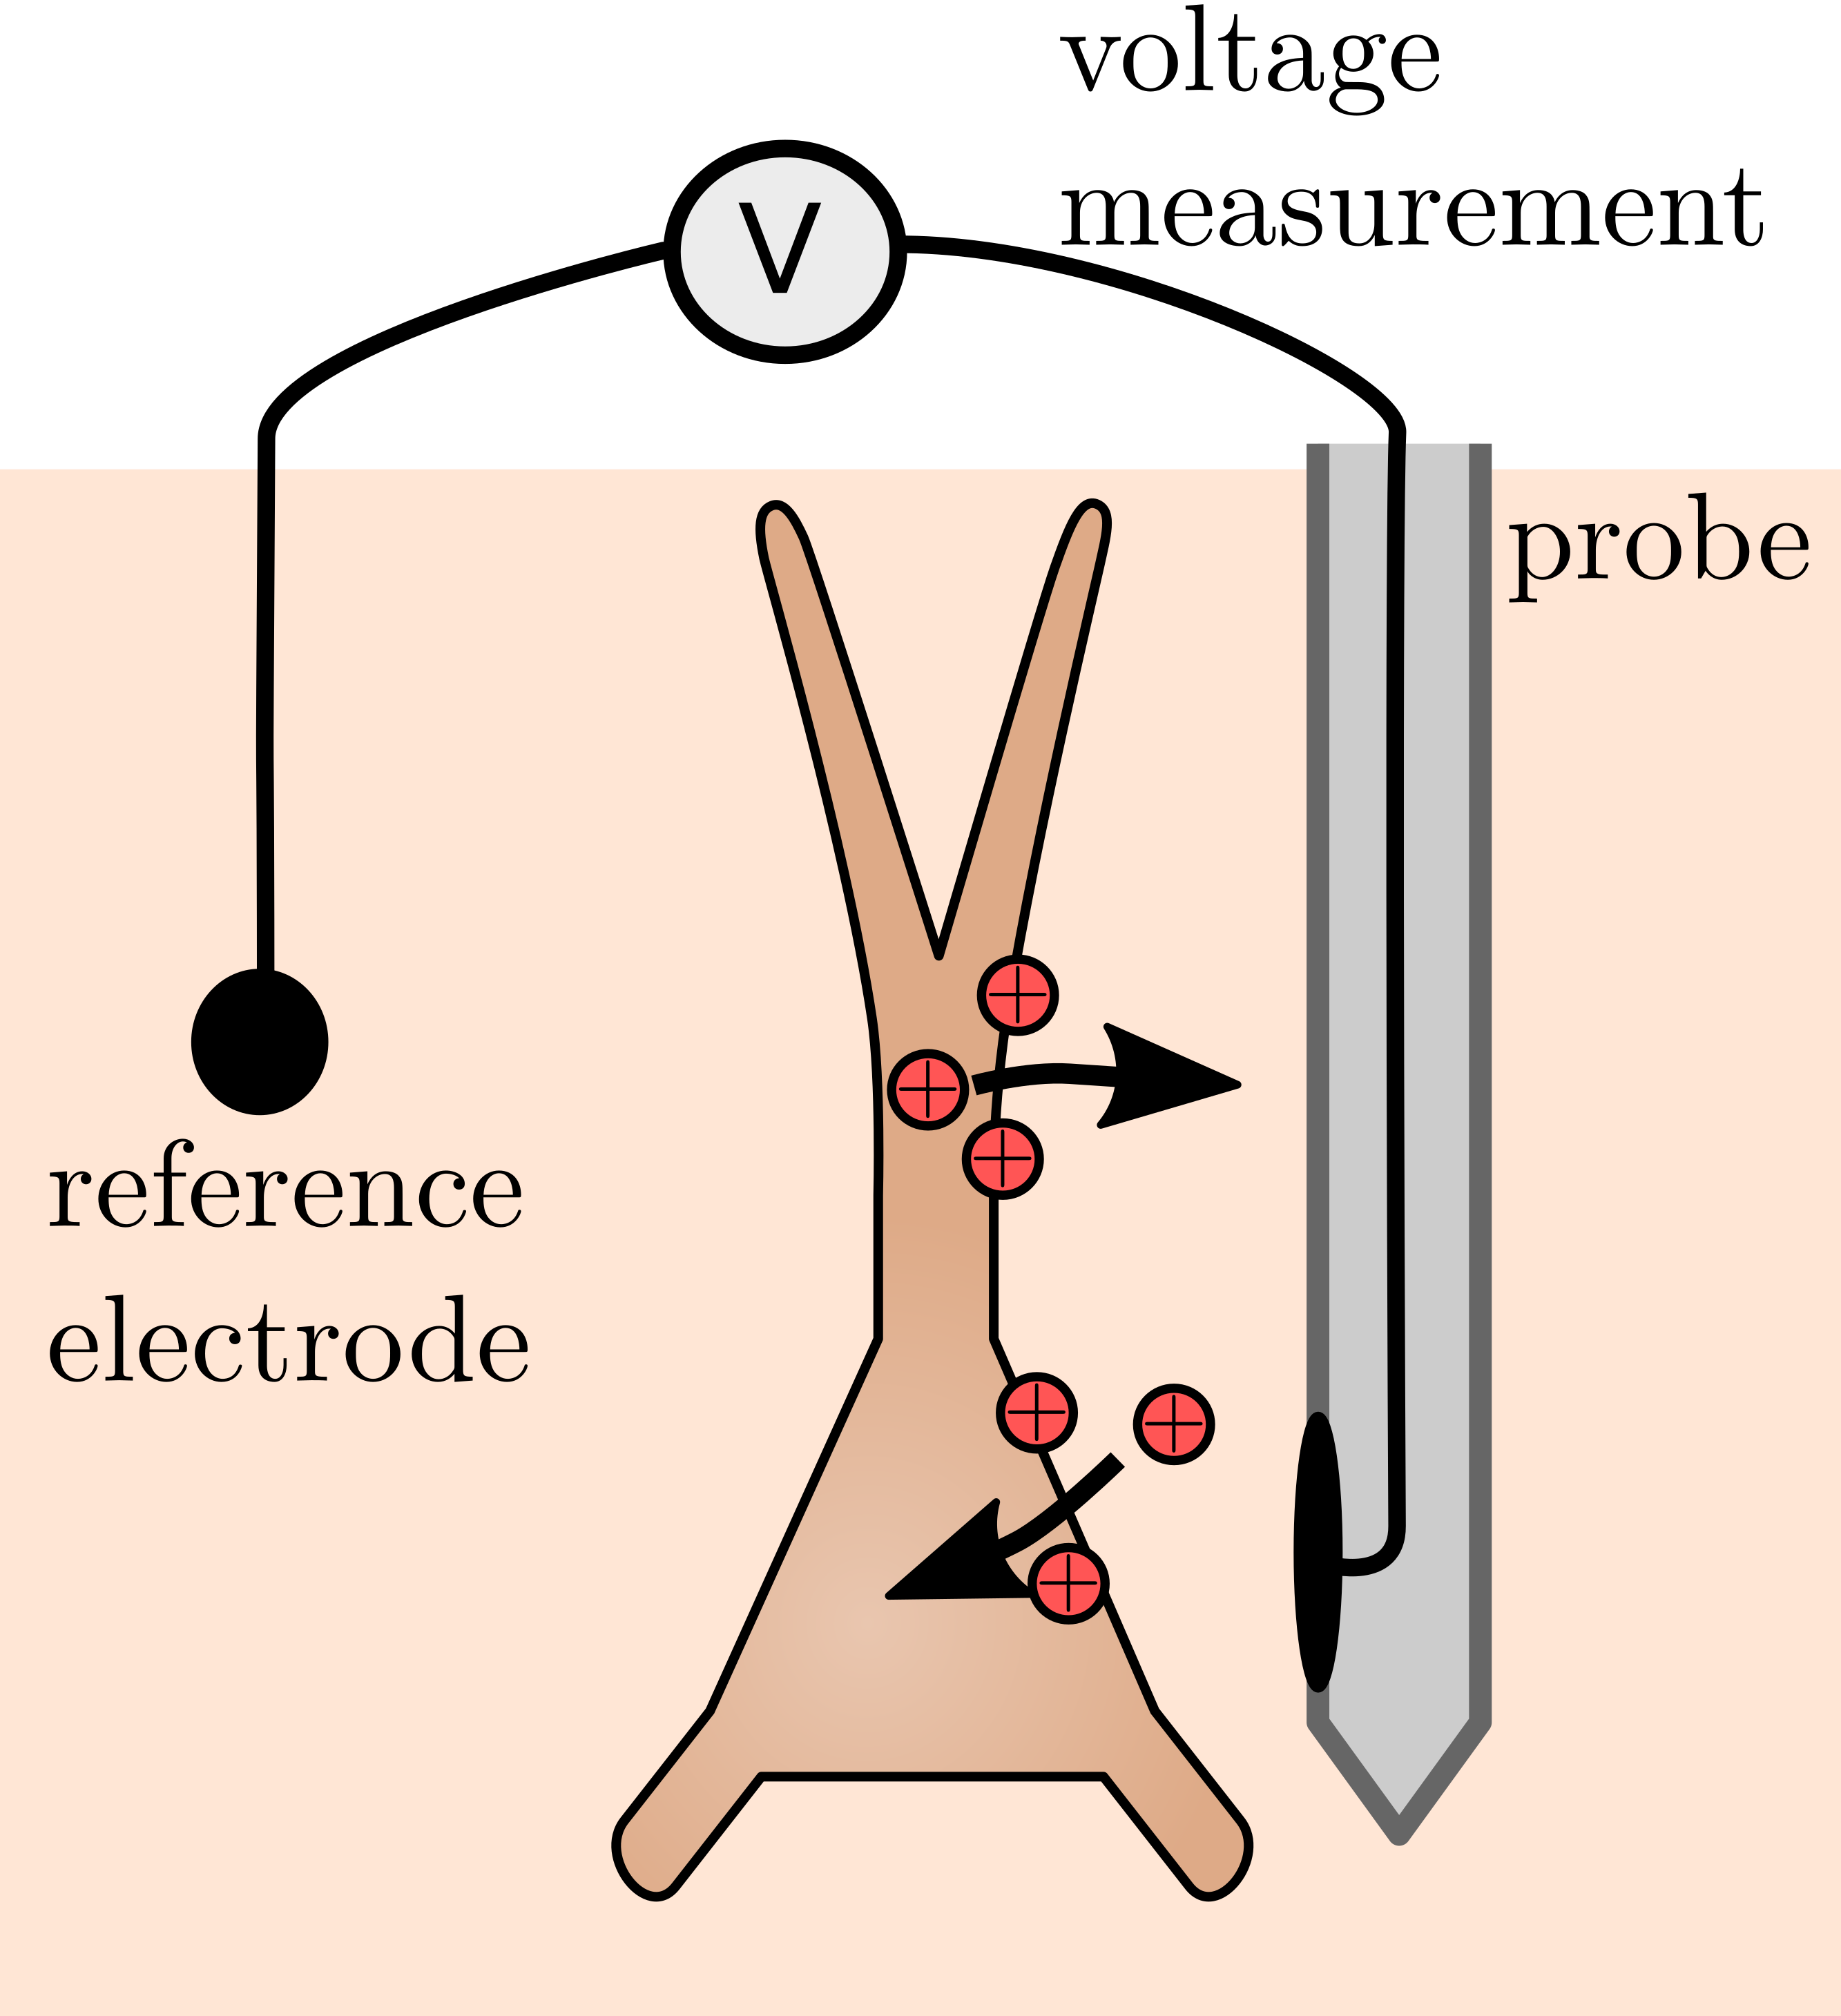
\includegraphics[width=0.4\textwidth]{Figures/Basics/rec_elec_circuit.png}
\end{center}
\caption[]{\textbf{Measurement of extracellular potential.}
Electric potential is measured between recording electrode (outside a neuronal soma) and reference electrode, and represents the energy required to move a positive test charge from the reference electrode to the measurement electrode. A positive current into the soma is leaving the extracellular medium in the vicinity of the recording electrode. Positive current will then flow into this region from elsewhere. The energy needed to move a positive charge to the measurement electrode (along with the "natural" current flow) is then negative.\tvnnote{Selve potensialet er jo V = J/C, og ikke J/A saa der maa vi snakke om ladninger? }
\ghnote{Enig med Torbjorn. Maa ha ladning for energitolkning. Stroem blir effekt. Hvor mange hestekrefter trenger elektroden?  Flyttet hit.}
}
\label{fig:Basics:elec_circuit}
\end{figure}

During the upstroke of the action potential, a (positive) Na$^+$ current flows into the neuronal soma, and thus leaves the extracellular region immediately outside it. Current conservation then implies that a positive current must be drawn into this region from elsewhere, or equivalently, that this region becomes an energy minimum that free charges will move towards. If we, with the electrode, try to move a positive charge into this region, we work along with the "natural flow" of charge, which means that the energy required is negative. This is why the upstroke of the action potential gives rise to a negative spike in the extracellular potential outside the neuron (more on this in \fref{chap:Spikes}). During the down-stroke of the action potential, a positive K$^+$ current leaves the neuron, and the situation is reversed. Extracellular currents will be directed away from the region where the electrode sits, and if we try to move a positive charge into this region, we must work against the "natural flow", and thus need to use energy. This is why the K$^+$ efflux gives rise to a positive spike in the extracellular potential outside the neuron.

The ampitude of the extracellular spike is inversely proportional to the extracellular conductivity. At first thought, this might seem counterintuitive. After all, if the conductivity is very low, a current can hardly propagate through the medium, and we might jump to the erroneous conclusion that also the amplitudes of the potential should be low. However, if we recall that the potential is a measure of the energy needed to push charges through that medium, the inverse proportionality makes sense: it requires more energy to push charges through a medium with low conductance than one with high conductance. This inverse proportionality is, of course, also what is stated by Ohm's law (\fref{eq:Basics:Ohm_3D_phi}). 

\tvntxt{The extracellular potential is really a measure of the energy needed to move a positive unit of charge from the reference electrode and to the measurement electrode (\fref{sec:Basics:interp_pot_charge}). If a positive current is leaving the extracellular region containing a measurement electrode (for example a sodium current flowing into a cell), then a positive current is drawn into the region, and the energy needed to move a positive charge here is negative (you can in theory gain energy) (\fref{fig:Basics:elec_circuit}). This is why the sodium peak of extracellular spikes is negative (\fref{chap:Spikes}). Slightly later, during the after-hyperpolarization phase of the spike, a potassium current is flowing out of the cell. Moving additional positive charges there now requires more energy, making the measured extracellular potential positive.

Many people (hvertfall Torbj\o rn) might have the intuition that if the extracellular conductivity is very low, the amplitude of the extracellular potential should also also be very low (after all "the signal can hardly propagate through the medium"). However, when a current source is pushing a current through a resistive medium, the drop in the potential will be proportional to the inverse of the conductivity (see Ohm's law), and therefore a lower conductivity gives a larger amplitude of the extracellular potential. 
%the extracellular potential is the energy needed to move a unit charge from a reference electrode to a measurement electrode, and therefore, if the extracellular conductivity is very low, more energy is needed.
\gen{Jeg synes det er lettere aa tenke/snakke om str{\o}mmer enn ladninger. Naar en str{\o}mkilde  presser en str{\o}m gjennom et Ohmsk medium saa blir det et spenningfall (hopp) i mediet som er proporsjonalt med motstanden. Men ladningene som flytter paa seg faar ikke mer energi, alle frigjort energi blir vel til varme i det ohmske mediet?} 
}


\subsection{\blue{Two-step approach for modeling extracellular potentials}}
\label{sec:Basics:twostep}
To compute extracellular potentials using \fref{eq:Basics:continuity2}, we need to know the neuronal output current source density $C$. Generally, the transmembrane currents in neurons depend on the membrane potential $V_\text{m}$, defined as the difference between the intracellular ($V_\text{i}$) and the extracellular ($V_\text{e}$) potentials immediately inside and outside the membrane. Hence, in principle, transmembrane currents depend on extracellular potentials, and the extracellular potential in turn depends on the transmembrane currents of all nearby neurons. As it is very challenging to simulate all these variables simultaneously in a self-consistent manner, standard modeling approaches are based on the simplifying assumption that the neurodynamics is independent of the extracellular potential. Since the transmembrane potential ($\sim -70$~\si{\milli\volt}) tends to be much bigger than extracellular potentials ($\sim 1 \,\si{\milli\volt}$), this is expectedly a reasonable approximation (but see \fref{sec:Neuron:HHCassumptions} for a further discussion). One may then take a two-step approach to model the cellular and extracellular dynamics:

\begin{itemize}
\item {\bf Step 1:} Compute the cellular dynamics (intracellular currents, membrane currents, and membrane potential) using a separate framework based on the assumption that this is independent on what goes on in the extracellular space (Fig. \ref{fig:Basics:Twostep}B).
\gen{Er det saa strengt? Kravet er vel bare at det som skjer i nevronene ikke skal paavirke det ekstracellulaere potensialet nevneverdig? Vi kan jo feks modellere elektrisk stimulering.}

\item {\bf Step 2:} Use the transmembrane currents computed in Step 1 as "external" input currents (sinks and sources) $C$ to the extracellular space (Fig. \ref{fig:Basics:Twostep}C). Based on \fref{eq:Basics:continuity2}, with $C$ as obtained in Step 1, an analytical formula can be derived for how the set of transmembrane currents give rise to an extracellular potential $V_\text{e}({\bf r})$.
\end{itemize}

Throughout this book, we shall use this two-step approach to compute extracellular potentials, but we will briefly introduce the theory behind alternative and more physically detailed frameworks. The standard framework for completing Step 1 is presented in \Fref{chap:Neuron}, and we will refer to it as the multicompartment (MC) framework, as it is based on multicompartment models of neurons. The standard framework for completing Step 2 is the volume conductor (VC) theory presented in  \Fref{chap:VC}.



\section{\blue{Maxwell's equations}}
\label{sec:Basics:Maxwell} \index{Maxwell's equations}
The physics of electromagnetism is summarized by Maxwell's equations, and we end this chapter by going briefly through these pillars of electromagnetism. We will also discuss some of the approximations of Maxwell's equations that we use when studying brain tissue.

Maxwell's equations come in two versions, referred to as the microscopic and macroscopic versions. The microscopic version is the most fundamental, but using it requires knowledge of the positions of all individual charges. Since that is unfeasible for any medium at a macroscopic level, we therefore only list up the macroscopic set of equations:

\begin{eqnarray}
{\bf \nabla}\cdot {\bf D} & = & \rho, \label{eq:Basics:Max11} \\
{\bf \nabla} \cdot {\bf B} & = & 0,   \label{eq:Basics:Max22} \\
{\bf \nabla} \times {\bf E} & = & - \frac{\partial {\bf B}}{\partial t},  \label{eq:Basics:Max33} \\
{\bf \nabla} \times {\bf H} & = & {\bf i}_\text{free} + \frac{\partial {\bf D}}{\partial t}.  \label{eq:Basics:Max44}
\end{eqnarray}
Here $\rho$ and ${\bf i}_\text{free}$ are the free (unbound) charge and current densities, respectively, as the influence of bound charge and current is incorporated in the auxillary displacement and magnetizing fields, ${\bf D}$ and ${\bf H}$. For linear mediums, ${\bf D}$ and ${\bf H}$ can be expressed in terms of the fundamental magnetic (${\bf B}$, with units tesla (\si{\tesla})) and electric (${\bf E}$) fields through the constitutive relations\index{Constitutive relations} ${\bf B} = \mu{\bf H}$ and ${\bf D} = \epsilon {\bf E}$, where $\mu$ (units henries per metre (\si{\henry\per\metre})) is the magnetic permeability of the medium and $\epsilon$ (units \si{\farad\per\metre}) the electric permittivity of the medium. By \textit{constitutive relations}, we simply mean relations that are observed experimentally to be good approximations for a specific material. They are known to be excellent approximations for brain tissue \cite**{Nunez2006}. Maxwell's equations then take the form:

\begin{eqnarray}
{\bf \nabla}\cdot {\bf E} & = & \frac{\rho}{\epsilon}, \label{eq:Basics:Max1} \\
{\bf \nabla} \cdot {\bf B} & = & 0,  \label{eq:Basics:Max2} \\
{\bf \nabla} \times {\bf E} & = & - \frac{\partial {\bf B}}{\partial t}, \label{eq:Basics:Max3} \\
{\bf \nabla} \times {\bf B} & = & \mu {\bf i}_\text{free} + \mu\epsilon\frac{\partial {\bf E}}{\partial t}.  \label{eq:Basics:Max4}
\end{eqnarray}

\Fref{eq:Basics:Max1} is Gauss's law (for electricity). The free charge density, $\rho$, can generally be non-zero, although we argued earlier that brain tissue for practical purposes can be assumed to be electroneutral at the coarse-grained scale.

\Fref{eq:Basics:Max2} is Gauss's law for magnetism, and is the magnetic equivalent to eq. \ref{eq:Basics:Max1}. Whereas \fref{eq:Basics:Max1} allows a spatial gradient of the electric field due to a local charge density $\rho$, \fref{eq:Basics:Max2} disallows the corresponding gradient in the magnetic induction field. That is because magnetic monopoles do not exist. 

\Fref{eq:Basics:Max3} is the Maxwell-Faraday equation for electromagnetic induction. The cross product ${\bf \nabla} \times {\bf E}$ represents a certain kind of change in the electric field called the \textit{curl}. The equation tells us that such a change will be induced if there is a temporal variation in the magnetic field.

\Fref{eq:Basics:Max4} is Ampere's circuital law, and is the magnetic equivalent to \fref{eq:Basics:Max3}. According to \fref{eq:Basics:Max4}, a magnetic field will be induced either by an electric current of free charges going through the medium (first term on the right), or by a temporal change in the displacement field (second term on the right). The last term is often called the displacement current. The Ohmic current that we introduced earlier (\fref{eq:Basics:Ohm_general}) is an example of a current of free charges, while the capacitive current that we introduced earlier (\fref{eq:Basics:Icap_mem}) is an example of a displacement current, where the capacitance can be expressed as a function of $\epsilon$.

It is interesting to note that the principle of current and charge conservation follows directly from Maxwell's macroscopic equations. To see this, we may start with taking the divergence (${\bf \nabla} \cdot$) of both sides of eq. \ref{eq:Basics:Max4}. Since the divergence of a cross product is always zero, \fref{eq:Basics:Max4} then reduces to:
\begin{equation}
{\bf \nabla} \cdot \left( {\bf i}_\text{free} +  \epsilon \frac{\partial {\bf E}}{\partial t} \right) = 0.
\label{eq:Basics:Max4dot}
\end{equation}
This equation states that the total current (${\bf i}_\text{tot} = {\bf i}_\text{free} +  \epsilon \frac{\partial {\bf E}}{\partial t}$) into any volume of space must be zero. To see the charge conservation explicitly, we can insert \fref{eq:Basics:Max1} for ${\bf E}$ to obtain:
\begin{equation}
- {\bf \nabla} \cdot {\bf i}_\text{free} =  \frac{\partial \rho}{\partial t}.
\label{eq:Basics:currentconservation}
\end{equation}
Hence, if the left hand side is nonzero, there is a net influx of free charges into a volume, and if that is the case, there must be an accumulation of charge there, as described by the right hand side of the equation. This equation thus reveals the equivalence between the displacement current (last term on the right hand side of \fref{eq:Basics:Max4dot})
\gen{Der staar det bare 0 :-)}  and a local accumulation of free charge (left hand side of \fref{eq:Basics:currentconservation}). \gen{Right hand side?}


\subsection{\blue{Quasi-static approximations of Maxwell's equation}}
\label{sec:Basics:Quasistatic} \index{Quasi-static approximation}
Together, Maxwell's equations give a unified theory for electricity and magnetism, and lay the theoretical fundament for understanding electromagnetic radiation such as light. We can "see the light" by looking at \fref{eq:Basics:Max3} and \fref{eq:Basics:Max4}. \Fref{eq:Basics:Max3} shows that a temporal change in the magnetic field induces an electric field perpendicular to the change (perpendicular, because that is what the curl-operation ${\bf \nabla} \times$ does), while \fref{eq:Basics:Max4} shows that a temporal change in the electric field (last term on the right hand side) induces a magnetic field perpendicular to the change. Electromagnetic radiation is due to such an interplay where electric and magnetic fields act on each other through a periodic series of inductions and cancellations that propagate as a wave through a medium. 

In principle, when neural activity generates an electric field, this electric field will again generate a magnetic field, which will again generate an electric field and so on. The generation of such electromagnetic waves are, however, a negligible feature of brain activity. Brain activity at the scale of tissue is therefore often studied using the quasistatic-approximations of Maxwell's equations \cite**{Hamalainen1993}. This means that in the calculation of ${\bf E}$ and ${\bf B}$, the source terms associated with temporal changes in the fields $\partial{\bf B}/\partial t$ and $\partial{\bf E}/\partial t$ are assumed to give a negligible contribution. When making these approximations, the electric and magnetic fields decouple. It is worth mentioning that the \textit{quasi-electrostatic} assumption that $\partial{\bf B}/\partial t \approx 0$ in \fref{eq:Basics:Max3} does not by necessity imply that the \textit{quasi-magnetostatic} assumption that $\partial{\bf E}/\partial t \approx 0$ in \fref{eq:Basics:Max4} must hold, or vice versa.

The CSD equation (\fref{eq:Basics:continuity2}) that we will use to describe electric fields in the brain rests heavily on the 
approximation that  $\partial{\bf B}/\partial t \approx 0$ in \fref{eq:Basics:Max3}, so that it simplifies to:
\begin{equation}
{\bf \nabla} \times {\bf E} \approx 0.
\label{eq:Basics:quasiel}
\end{equation}
A zero curl of the electric field is a prerequisite for expressing ${\bf E}$ as a gradient of a potential, like we did in \fref{eq:Basics:EV}. This approximation has been justified in many works, and is warranted because fields of physiological origin are normally of frequencies below a few thousand \si{\hertz}, and then have a negligible effect on electric fields \cite**{plonsey1967,Hamalainen1993,Bossetti2008,Gratiy2017}. 
 
In addition, the CSD equation rests on the approximation that the (static) magnetic fields are too small to significantly affect the movement of electric charges. As we briefly mentioned early in this chapter, charges can be accelerated both by electric and magnetic forces, collectively referred to as the Lorenz force:
\begin{equation}
{\bf F} = q({\bf E} + {\bf u}\times{\bf B}),
\label{eq:Basics:Lorenz}
\end{equation}
which adds a magnetic force to the electric force that we defined previously in \fref{eq:Basics:E}. Here, {\bf u} (units \si{\metre\per\second}) is the velocity of the charged particle, and the magnetic force is given by the cross product of the vectors ${\bf u}$ and ${\bf B}$, which means that it will act in the direction perpendicular to both of them. 

According to \fref{eq:Basics:Lorenz}, magnetic effects on the movement of charges will be negligible if 
\begin{equation}
\frac{uB}{E} \ll 1, 
\label{eq:Basics:LorenzCriterion}
\end{equation}
where we are thinking "large-scale", so that $u$ represents the averaged movement of charged particles in some preferred direction, whereas $E$ and $B$ represent typical electric and magnetic field strengths in brain tissue. Geomagnetic fields near the surface of the earth ($\sim 50 \, \si{\micro\tesla}$) are about $10^8$--$10^9$ as strong as neuromagnetic signals ($\sim 100 \, \si{\femto\tesla}$ \cite**{Hamalainen1993}). As the magnetic permeability ($\mu$) of brain tissue is about the same as in free space \cite**{Hamalainen1993}, \gex{the} magnetic field inside the brain will therefore be roughly the same as in the external world. In contrast, the electric conductivity of brain tissue ($\sim 0.3 \, \si{\siemens\per\metre}$) is about $10^{11}$ times higher than for air. The atmospheric electric fields on the surface of the earth ($\sim 100 \, \si{\volt\per\metre}$), will therefore only give a field contribution $\sim 10^{-9} \, \si{\volt\per\metre}$ in the brain, which is much smaller than the fields of neuronal origin ($\sim 1 \, \si{\volt\per\metre}$ \cite**{Cordingley1978}).  Inserting $E = 1 \, \si{\volt\per\metre}$ and $B = 50 \, \si{\micro\tesla}$ into \fref{eq:Basics:LorenzCriterion}, the criterion for magnetic effects on the movement of charges to be negligible is that:
\begin{equation}
u \ll 2\times10^4 \,\si{\metre\per\second}.
\label{eq:Basics:LorenzCriterion2}
\end{equation}

As we explained in \fref{sec:Basics:Note}, the drift velocity of ions due to volume currents in brain tissue is \gex{on} the order of nanometers per second.  The maximal bulk flow of ions in the brain is therefore probably due to blood flow. As blood is electroneutral, it does not carry any net charge, but it does carry positive and negative ions in a given direction, and a magnetic field would to bend off the oppositely charged ions in opposite directions. However, the maximal flow velocity in arteries has been estimated to $\sim 1 \,\si{\metre\per\second}$ \cite**{bishop1986}, \gen{Synes det er mye space i enhetene som si-pakka produserer} which is by far slow enough for such magnetic effects to be neglected. Even thermal velocities $u \sim (k_BT/m)^{1/2} \approx$ 100 --1000 \si{\metre\per\second} of ions in a body tempered brain would be too slow to violate the criterion in \fref{eq:Basics:LorenzCriterion2}). We note, however, that the thermal velocity is not really a candidate for insertion into \fref{eq:Basics:LorenzCriterion2}, since it represents the average absolute velocity of randomly walking particles, and therefore does not give rise to any net movement of charges on the system level, i.e., magnetic forces acting on particles moving in one direction will be cancelled by forces acting on particles in the opposite direction and so on. Like we have assumed throughout this chapter, we therefore can conclude that magnetic effects on the movement of charges in brain tissue are negligible.  The reason why this is important, is that ${\bf i}_\text{free}$ in \fref{eq:Basics:Max4dot} then becomes independent of ${\bf B}$, which we implicitly assumed when we used Ohm's law for volume conductors (\fref{eq:Basics:Ohm_3D_phi}) to derive the CSD equation (\fref{eq:Basics:continuity2}).

\ghnote{Har brukt irriterende mye tid paa de to siste avsnittene. Irriterende - fordi jeg ikke en gang vet om det er lurt aa ha med saa mye om dette. Mye plass paa noe som kanskje kun er av hypotetisk relevans.  Har foroevrig utregninger av drifthastigheter ogsaa paa lur (utkommentert tekst), hvis noen skulle vaere interessert i det.}

\ghnote{Gaute foreslo at relevant ligning er $F_B = BI\ell$, men hva gir det oss? For det foerste, saa tenker vi oss ikke en kabel med lengde $\ell$, men en volumstroem, saa det blir uklart hva kraften da er en kraft paa: Kraft paa stroemmen i en gitt retning? Sier ikke det oss ca. det samme som kraft per enkeltladning hvis det finnes en gjennomsnittshastighet $u$? For det andre, hvis vi tenker oss at kabelen vaar er blodaaren, saa gaar det ingen stroem der, da blodet er elektronoeytralt.}

\gen{Litt usikker paa siste utsagn. Elektriske kobberkabler er jo ogsaa elektrisk noytrale, men der kan det gaa strom. Men det du mener er kanskje at det ikke kan gaa en strom hvis du baerer en kobberkabel rundt i huset?}

\ghnote{Rikig: Det vil ikke gaa stroem hvis jeg baerer en kobbeerkabel rundt i huset, saa sant jeg ikke har gnidd den mot en ullgenser foerst. Paa samme maate gaar det ikke elektrisk stroem gjennom blodårer bare fordi blod pumpes gjennom dem, så sant ikke jeg har gnidd blodet mot en ullgenser foerst. Men: selv om det ikke gaar netto stroem i blodet, frakter det jo positive og negative ioner. Et B-felt vil da boye av K$^+$ og Cl$^-$ i motsatte retninger, og vi kan tenke oss ladningsseparasjon, at positive og negative ioner vandrer langs hver sin vegg av blodaaren. Dette gir ingen netto kraft paa blodaaren, men ville sikkert kunne gitt en spennende felt-effekt hvis effekten var stor. I hjernen er den, jmf. utregningen over, veldig liten i forhold til effekter skapt av E-felter. }  

%To make an estimate the ratio between electric and magnetic forces in the brain, we need to insert some relevant value for the velocity (${\bf u}$) in \fref{eq:Basics:Lorenz}. As candidates, we could imagine using (i) the thermal velocity of ions moving in the saline solution of the brain, (ii) the drift velocity of ions carrying electric current through the saline solution, or (iii) a bulk flow of the solution that the ions live in. The thermal velocity (i), ${\bf u}_\text{therm} \sim (k_BT/m)^{1/2} \approx$ 100 --1000 \si{\metre\per\second}, is not really a candidate. Since it is the average absolute velocity of randomly walking particles, it has no preferred direction, meaning that forces acting on particles moving in one direction will be cancelled by forces acting on particles in the opposite direction. The drift velocity (ii) due to an extracellular current density, can be calculated from 

%${\bf u}_\text{drift} = \sigma_\text{t} E/(-e[q]n_A)$. Here, $e$ is the unit charge and $N_A$ Avogadros number. If we use typical values for brain tissue, assuming a conductivity $\sigma_\text{t} = 0.2 \si{\siemens\per\metre}$, a field strength $E\sim 1 \si{\volt\per\metre}$ a concentration of charge carriers $[q] \sim 300 \si{\milli\molar}$, we get an estimate $v_{drift} \sim 10 \si{\nano\metre\per\second}$. This is a very small velocity, so our main candidate will be the bulk flow (iii). Since the bulk solution on the brain is electroneutral, advective bulk flow does not carry any net charge. However, it does carry positive and negative ions in a given direction, and a magnetic field bend the oppositely charged ions in opposite directions. The maximal blood flow velocity through arteries has been estimated to be ${\bf u}_\text{bulk} \sim 1 \,\si{\metre\per\second}$ \cite**{bishop1986}, and we may take this s an upper limit for a the bulk flow velocity in the brain. 

%If we combine a bulk flow velocity of $\sim 1 \,\si{\metre\per\second}$ with the geomagnetic field $B \sim \times10^{-4} \, \si{\tesla}$ \cite**{Hamalainen1993}, and the typical $E = 1 \,\si{\volt\per\metre}$ \cite**{Cordingley1978} arising from neural activity, we can estimate the ratio between the magnetic and electric force to be $uB/E \sim 10^{-4}$. Hence, as we have assumed throughout this chapter, magnetic effects on the movement of charges in brain tissue are negligible. The reason why this is important, is that ${\bf i}_\text{free}$ in \fref{eq:Basics:Max4dot} then becomes independent of ${\bf B}$, which we implicitly assumed when we used Ohm's law for volume conductors (\fref{eq:Basics:Ohm_3D_phi}) to derive the CSD equation (\fref{eq:Basics:continuity2}). Together, the assumptions that ${\bf \nabla} \times {\bf E} \approx 0$ and $uB \ll E$ are sufficient for electric and magnetic fields to decouple.

%\ghnote{Svar til Torbjorn: Fordi den er skikkelig liten. $I = \sigma E A = e^{-}n_eAv_{drift}$. For typiske verdier i hjernen, $\sigma = 0.2$ S/m og $E\sim 1$ V/m, $n_e \sim 300$ mM $= 300 N_A$ per kubikkmeter (sum av alle konsentrasjoner, antar valens 1),beregnet jeg $v_{drift} \sim 6$ nm/s, som er mye lavere enn blod-hastigheten. I foelge regneeksempler paa nettet er drifthastigheten for 20 A i kobberkabel typisk paa noen titalls micrometer/s. Med andre ord vil blodstroem dominere. Skal vi ta med regneeksempler paa dette?} 

Of the assumptions underlying the quasi-static approximation, the approximation that $\partial{\bf E}/\partial t \approx 0$ in \fref{eq:Basics:Max4} is the weakest point \cite**{plonsey1967,Bossetti2008}. It has been shown to be a fairly good approximation for large scale brain activity \cite**{plonsey1967,Hamalainen1993}, but does not apply to finer spatial scales, as it is the displacement term that gives rise to the capacitive charging of neural membranes \cite**{Gratiy2017}. Importantly, the approximation that $\partial{\bf E}/\partial t \approx 0$ is not a requirement for using the CSD equation on the form (\fref{eq:Basics:continuity2}), as possible capacitive components of the tissue current can be accounted through using a complex tissue conductivity $\sigma_t$ (see \fref{chap:Sigma}). \gen{Dreier dette avsnittet seg om hele brain tissue eller bare ECS?}


